
%%%%%%%%%%%%%%%%%%%%%%% file typeinst.tex %%%%%%%%%%%%%%%%%%%%%%%%%
%
% This is the LaTeX source for the instructions to authors using
% the LaTeX document class 'llncs.cls' for contributions to
% the Lecture Notes in Computer Sciences series.
% http://www.springer.com/lncs       Springer Heidelberg 2006/05/04
%
% It may be used as a template for your own input - copy it
% to a new file with a new name and use it as the basis
% for your article.
%
% NB: the document class 'llncs' has its own and detailed documentation, see
% ftp://ftp.springer.de/data/pubftp/pub/tex/latex/llncs/latex2e/llncsdoc.pdf
%
%%%%%%%%%%%%%%%%%%%%%%%%%%%%%%%%%%%%%%%%%%%%%%%%%%%%%%%%%%%%%%%%%%%


\documentclass[runningheads,a4paper]{llncs}

\usepackage{listings}
\usepackage{amssymb}
\usepackage{graphicx}
\usepackage{longtable}
\usepackage{url}
\usepackage{xcolor}
\usepackage{acro}


\newcommand{\keywords}[1]{\par\addvspace\baselineskip
\noindent\keywordname\enspace\ignorespaces#1}
\usepackage{nameref}
\acsetup{first-style=short}

% Abbreviations
\DeclareAcronym{dp}{short = DP, long = Draw Pile Module, class = abbrev}
\DeclareAcronym{fp}{short = FP, long = Foundation Pile Module, class = abbrev}
\DeclareAcronym{tp}{short = TP, long = Tableau Pile Module, class = abbrev}
\DeclareAcronym{p}{short = P, long = Player Module, class = abbrev}
\DeclareAcronym{pb}{short = PB, long = Player Bot Module, class = abbrev}
\DeclareAcronym{fifo}{short = FIFO, long = First In First Out (Queue), class = abbrev}
\DeclareAcronym{lifo}{short = LIFO, long = Last In First Out (Stack), class = abbrev}
\DeclareAcronym{gui}{short = GUI, long = Graphical User Interface, class = abbrev}
\DeclareAcronym{mc}{short = MC, long = Module Connector, class = abbrev}

% Nomenclature
\DeclareAcronym{card}{short = card, long = (In the Petri Net context) A token with a color which represents a card in the deck., class = nomencl}
\DeclareAcronym{command}{short = command, long = A token with a color which represents a turn or movement command., class = nomencl}
\DeclareAcronym{destroyer}{short = destroyer, long = A transition which only has inputs. Opposite of generator., class = nomencl}

\newcommand{\GPenSIM}{../GPenSIM}
\definecolor{matlabcomment}{RGB}{34,139,34}
\definecolor{matlabstring}{RGB}{160,32,240}
\definecolor{matlabkeyword}{RGB}{0,0,255}
\lstdefinestyle{matlabcode}{
	language=Matlab,
	frame=single,
	%caption=\lstname,
	stringstyle=\color{matlabstring},
	keywordstyle=\color{matlabkeyword},
	commentstyle=\color{matlabcomment},
	basicstyle=\fontsize{6}{7}\selectfont,%\tiny
	breaklines=true,
	numbers=left
}


\begin{document}
\mainmatter  % start of an individual contribution
% first the title is needed
\title{DAT530\\Discrete Simulation and Performance Analysis\\Final Project\\Solitaire game strategy}
% a short form should be given in case it is too long for the running head
\titlerunning{DAT530 - Final Project}
\author{Racin W. Nygaard}
\authorrunning{DAT530 - Final Project - Solitaire game strategy}
% (feature abused for this document to repeat the title also on left hand pages)
\institute{Universitetet i Stavanger}

\toctitle{Abstract}
\tocauthor{ }
\maketitle
	


\begin{abstract}
This report describes the final project in DAT530. The topic of the project was chosen to be the game Solitaire. The goal of the project was to model the whole game, and perform analysis on the game strategy. To ease the testing of the model, a fully functional GUI was also developed. This GUI can be used to play a game of solitaire. The report contains description of the developed model, the newly created functions, the GUI, analysis of the model and the results.

\end{abstract}

\setcounter{tocdepth}{3}
\setcounter{secnumdepth}{3}

\tableofcontents
\listoffigures
\listoftables
\printacronyms[name=Abbreviations,include-classes=abbrev]
\printacronyms[name=Nomenclature,include-classes=nomencl]
\section{Introduction}
This project aims to study the popular card game, Solitaire[Site]. Solitaire is bundled with most Windows[Site] installations, as well as being available for free on several sources. It is also easy to play the game with a physical card deck. A detailed explanation of the games rules can be found in chapter \ref{sec1:solitaire_rules}, Solitaire Rules
\newline
Since the game utilizes all 52 cards of the deck, the number of possible initial game states is 52!, which is a very high number. A large number of these inital game states can be merged, as they offer no difference in the difficulty to solve. Some of these initial states are unsolvable, but even given a solvable game state, one often find oneself in an unsolvable game state, due to certain actions in the game are non-reversible,. There has been attempts to find the distribution of solvable and unsolvable initial game states [ref]. This is roughly 75 percent are solvable, however the study also shows that only 35 percent of the games are won by an experienced player.
\newline
This project contains a complete model of the game, a GUI to play the game, and a basic bot to simulate user actions. 

\subsection{Solitaire Rules}
\label{sec1:solitaire_rules}
Klondike, or Solitaire as it has been called in North America, is one of the most popular patience games.
\newline
 The game became very popular in the 19th century and the name Klondike is believed to have originated from the prospectors that were mining for gold in the Klondike region in Canada.
 \newline
 
Solitaire is played with a standard deck of 52 cards and no Jokers.
We will describe the layout and rules of the game 
\newline

 At the beginning of the game, the deck is shuffled and the cards are laid out in seven tableau piles from left to right. Each pile contains one additional card compared to the previous one. 
 There is one upturned card at the beginning of each pile. The first pile to the left contains one card facing up, the second contains one card facing down and one up, the third pile contains two cards facing down and one up, continuing to the seventh pile respectively, which contains six cards facing down and one facing up.
 Tableau piles can be built down by alternating colors. Partial or complete piles can be moved on top of other piles as long as long as the constraint of alternating card color is respected. 
 Empty piles can be filled with a King or a pile of cards that starts with a King.
\newline
 
We build up the piles by stacking cards of the same suit starting from Ace and finishing with King. The aim of the game is to build up a stack of cards of the same suit. When this is accomplished, the goal is to move this stack to foundation where the Ace of the suit had previously been placed. 
\newline
  
The remainder of the deck is dealt by turning one card at a time from the draw pile.
When all the cards from the draw pile have been turned, the draw pile can be reset. 
 
The layout of the piles is illustrated in figure \ref{fig:illuatration_solitaire}.
\begin{figure}
	 % Left, Bottom, Right, Top
	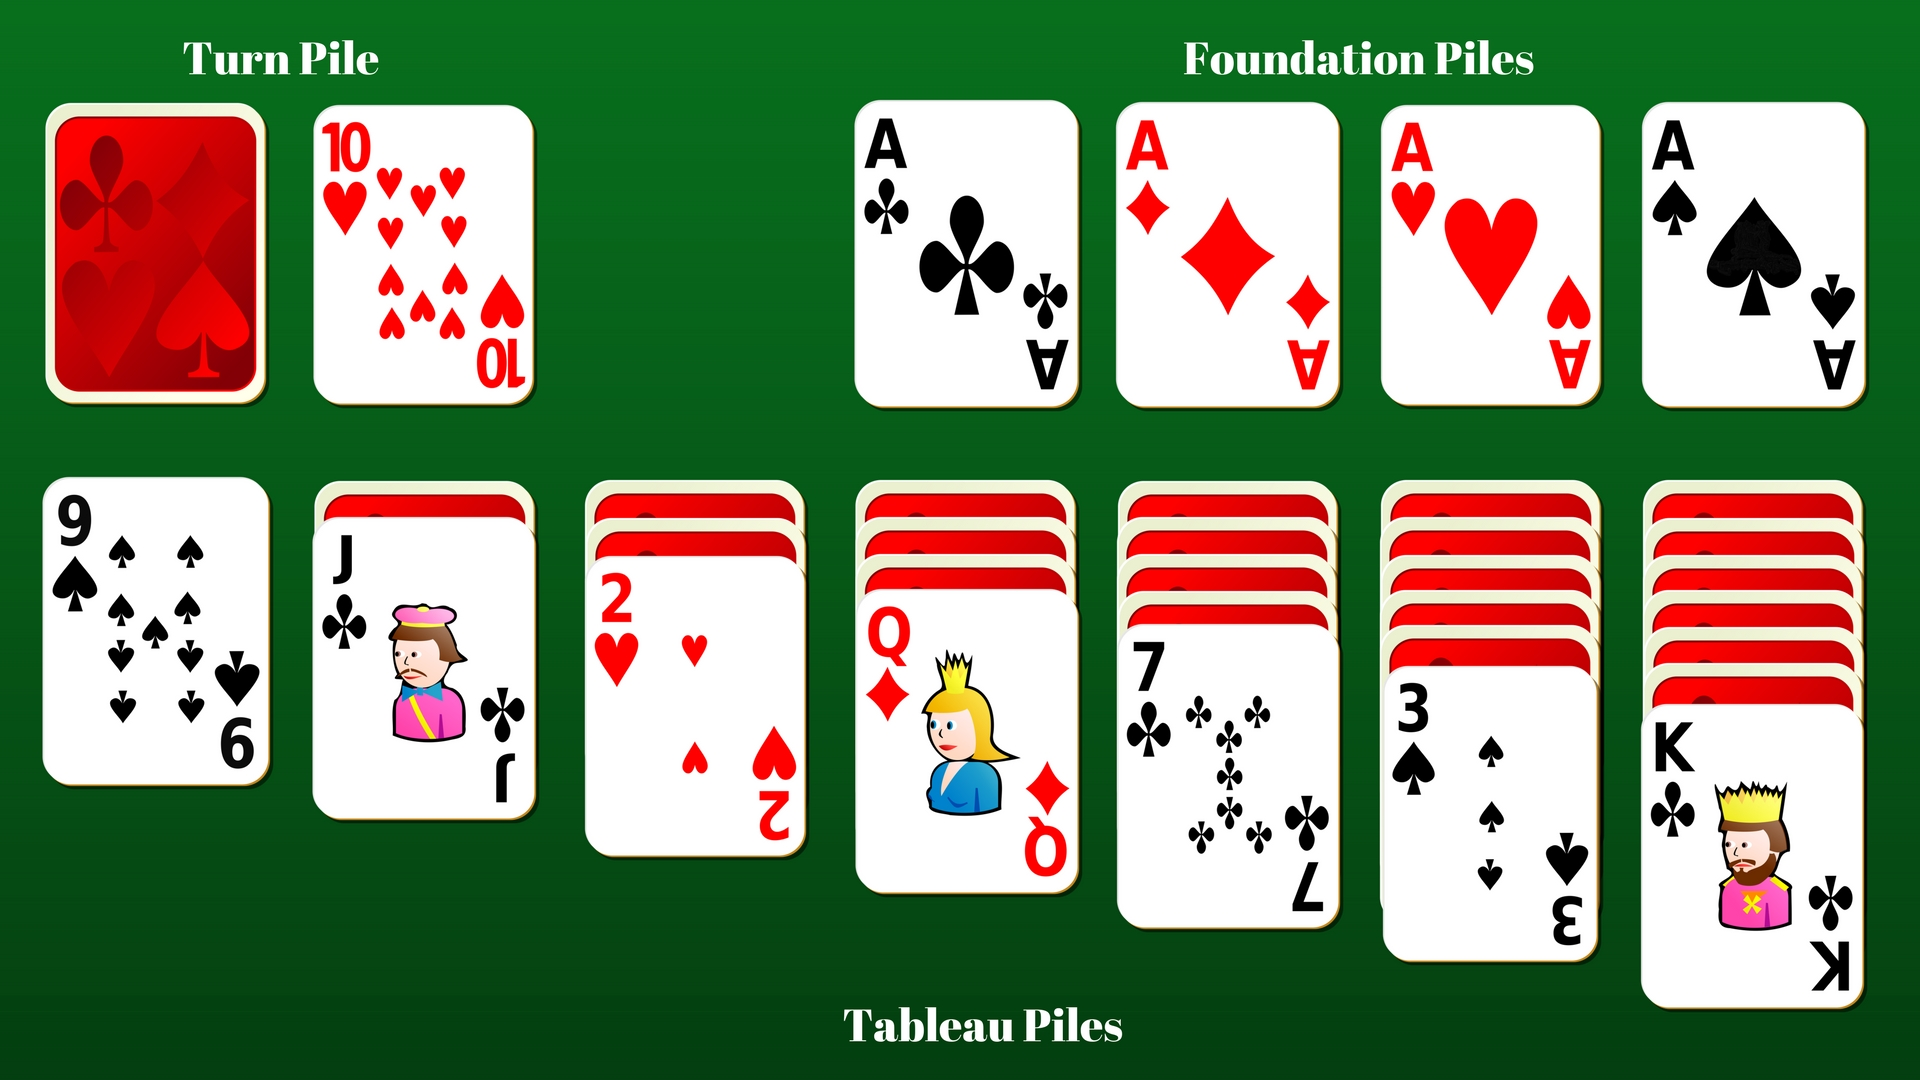
\includegraphics[trim=150 0 0 0, scale=0.3]{images/TableauPiles}
	\caption{Illustration of card layout in Solitaire}
	\label{fig:illuatration_solitaire}
\end{figure}

\clearpage
\section{Method and Design}
\label{sec:2_method_and_design}
\subsection{Naming Policy}
\label{sec:2_naming_policy}
The names of all transitions and places respects the restriction described in \cite{GPenSIMguide}, which states that only the 10 first characters of the names are significant. Acknowledging this, the first name of an element is always \textbf{t} or \textbf{p}, which means transition or place, respectively. \\

Next, the abbreviated name of the module will follow. The possibilities are \textbf{\ac{dp}, \ac{fp}, \ac{mc}, \ac{p}, \ac{pb},} and \textbf{\ac{tp}}. After this, either an underscore, \textbf{i} or \textbf{e} follow. The letter \textbf{i} means it's an internal transition, and \textbf{e} means it's and external transition. This is significant, as without these letters, the transitions \verb!tTPi_1_Move_Multiple! and \verb!tTPe_1_Move! would have a name collision. After either letter a underscore follows.\\

After the first underscore, the unique identifier will follow for the Tableau- and Foundation modules. The valid identifiers for \ac{tp} is \textbf{1, 2, 3, 4, 5, 6, 7}, and for \ac{fp} it is \textbf{Clubs, Diamonds, Hearts, Spades}. After the unique identifier another underscore will follow.\\

Lastly, a short descriptive name for the place or transition is appended.
\subsection{File structure}
\label{sec:2_file_structure}
To reduce the number of files, most of the pre- and post-processor files of the \ac{fp} and \ac{tp} modules have been combined in one single file. An example of this can be shown in listing \ref{lst:COMMON_PRE}, which shows parts of \verb!COMMON_PRE!
\lstinputlisting[style=matlabcode,caption=COMMON\_PRE.m lines 1-5,label=lst:COMMON_PRE,lastline=5]{\GPenSIM/COMMON_PRE.m}

By doing this it is possible to reduce the number of files required without overloading the \verb!COMMON_PRE! and \verb!COMMON_POST! files. It also makes it much easier to work and maintain the code as the logic is only located in one place, as opposed to four or seven places if each transition had their own file.
\newline

With this approach it is no longer possible to hard-code the names of the related transitions and places, so two additional functions; \verb!get_tableau_from_transname! and \verb!get_suit_from_transname! were developed. These functions take the name of the transition as input, and then return the unique identifier for which module it belongs to. The actual code is pretty simple, and parts of \verb!get_suit_from_transname! is shown in listing \ref{lst:get_suit_from_transname}. The reasoning behind not using the Matlab command \verb!contains! is simply that it is not supported in older versions.
\lstinputlisting[style=matlabcode,caption=get\_suit\_from\_transname.m lines 7-17,label=lst:get_suit_from_transname,firstline=7,lastline=17]{\GPenSIM/get_suit_from_transname.m}
\clearpage
\subsection{Overall Design}

\begin{figure}
	\begin{center} % Left, Bottom, Right, Top
		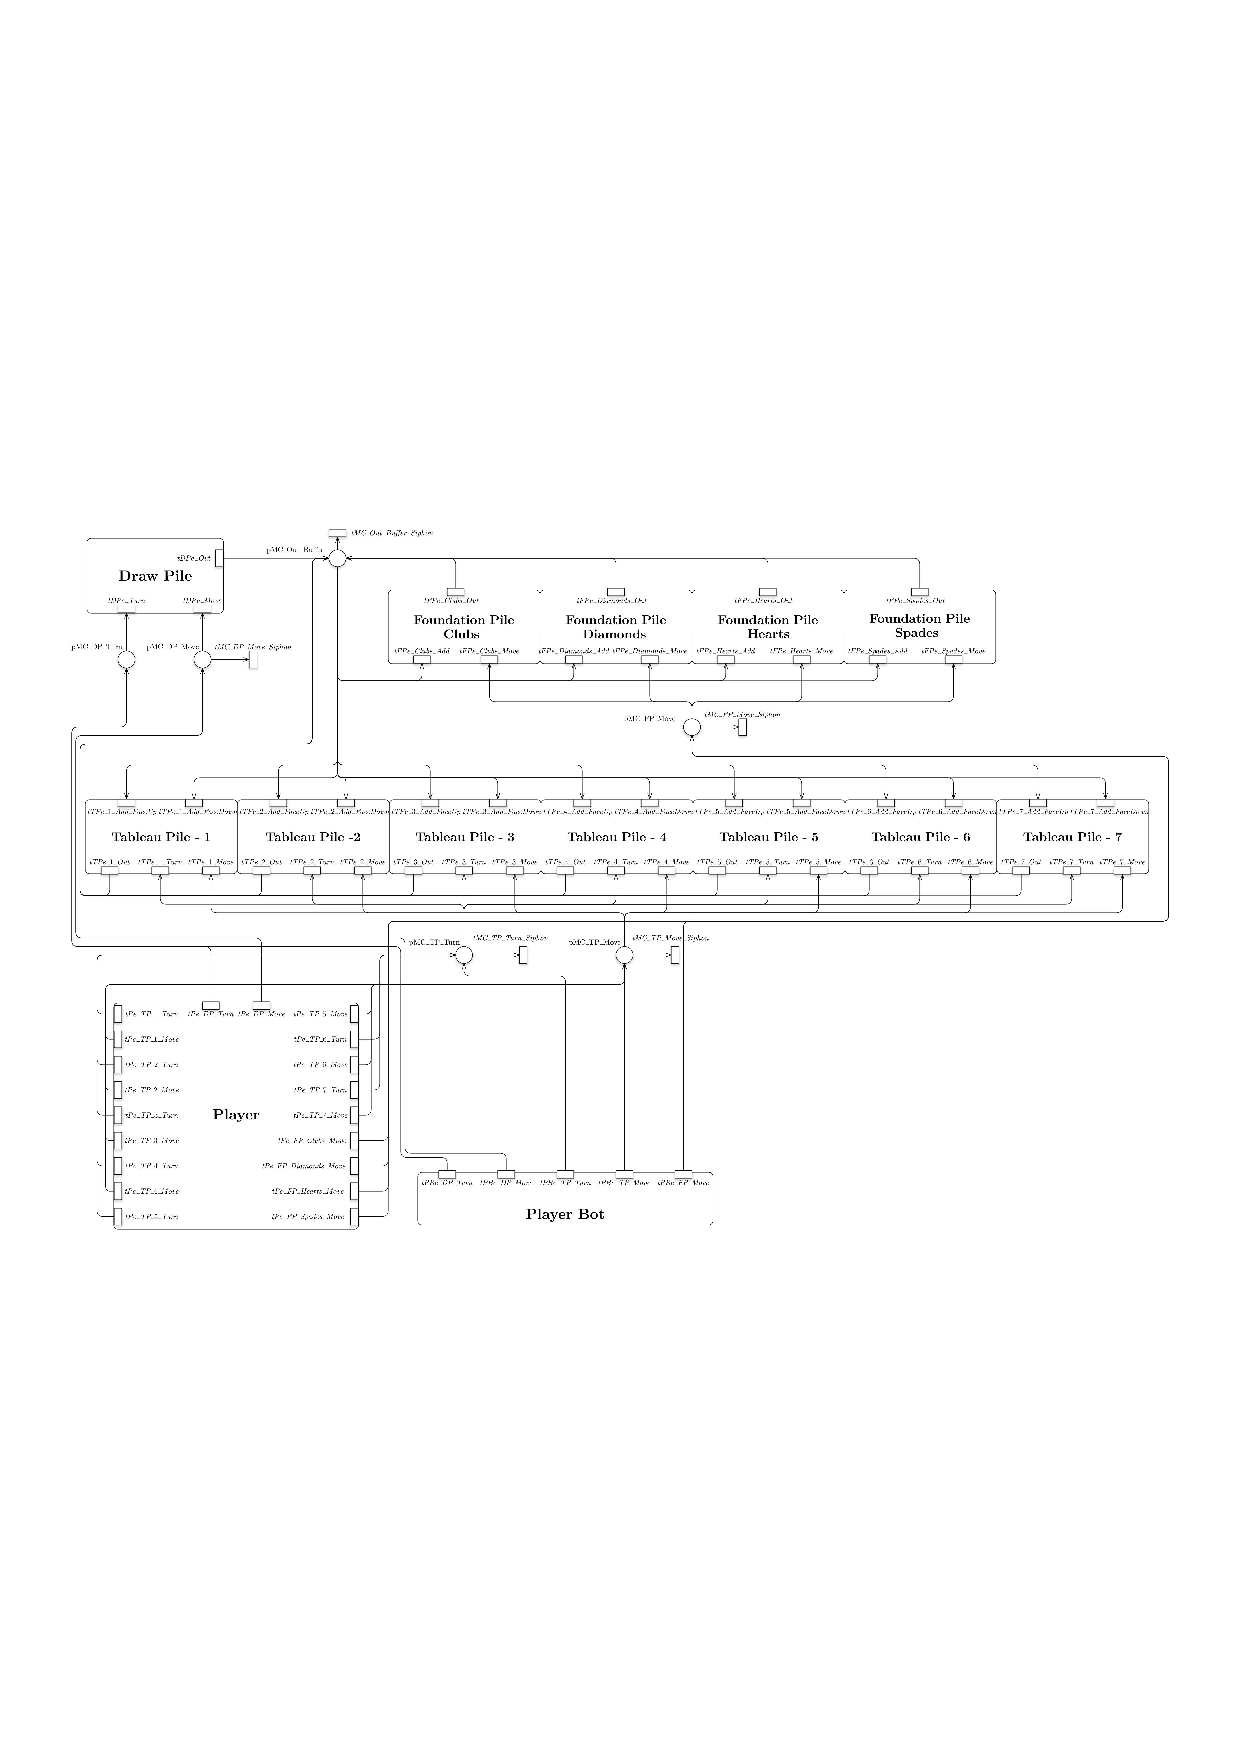
\includegraphics[trim=250 260 230 330,scale=1.1]{images/overallViewPdf}
		\caption{The complete model - Without the internal components of the modules.}
		\label{fig:full_horizontal}
	\end{center}
\end{figure}


The model is developed using a Colored Petri Net, and relies heavily on colors to represent the different card in the deck, and also to facilitate the communication between the different modules. The whole is quite large, containing 94 transition and 42 places. It is developed using the modular approach, and encompasses 6 different modules. Some of the modules are duplicated, with the only difference being the names of the transitions and places.
\clearpage
\subsection{Draw Pile Module}
\label{sec:draw_pile}
\begin{figure}
	\begin{center}
		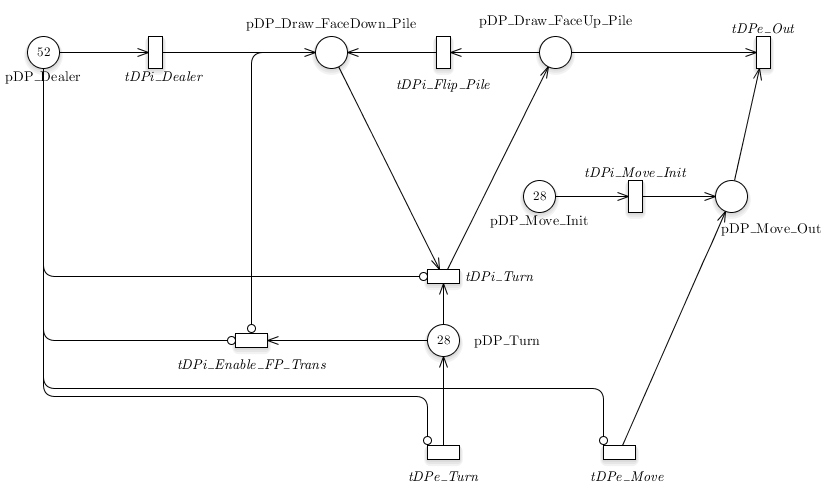
\includegraphics[width=\textwidth]{images/drawPile}
		\caption{Draw Pile Module}
		\label{fig:draw_pile}
	\end{center}
\end{figure}
The Draw Pile module is depicted in figure \ref{fig:draw_pile}, and has several key responsibilities, once of which is to do the initial dealing of cards. In order to preserve the correctness of the gameplay, external input is not allowed during this phase. When first running the model, all the initial tokens of \verb!pDP_Dealer! will be sent to \verb!tDPi_Dealer!. This transition will give each token a color which represents a \ac{card} in the deck. Possible colors are initially stored in the cell \verb!global_info.DECK!. If \verb!global_info.RANDOM_DECK! is set, a random permutation of the colors will be given to the tokens. By having \verb!global_info.RANDOM_DECK! set to false, it is possible to run analytics which require that the cards are dealt equally each time.
\newline

After all tokens are given a color, \verb!tDPi_Turn! will be enabled. This transition will move cards from the pile which represents face-down cards, \verb!pDP_Draw_FaceDown_Pile! to the one representing face-up cards, \verb!pDP_Draw_FaceUp_Pile!. This transition will fire as many times as the length of \verb!global_info.INITIAL_DEAL_MOVE!, which is 28 in a normal game. This is not something that would be done if the game where played with physical cards, as they would just be dealt without turning them. In this model however, this is required so that existing logic could be re-used.
\newline

Concurrently to the firing of \verb!tDPi_Turn!, the transition \verb!tDPi_Move_Init! will fire an equal amount of times. The transition will give each of the tokens in \verb!pDP_Move_Init! a color which represents to which tableau pile the \ac{card} should be moved to. The color given to each token is augmented by the cell, \verb!global_info.INITIAL_DEAL_MOVE!. An example of a color given is \emph{Move:\ac{tp}1:\ac{dp}} which means; \textit{Moving a card from source DP to destination \ac{tp}1}. Every time a \ac{card} reaches its destined tableau pile, the variable \verb!global_info.CARDS_DEALT! will be incremented by one in \verb!COMMON_POST!. Once it becomes equal to the length of \verb!global_info.INITIAL_DEAL_MOVE!, the initial dealing phase is over, and the normal phase starts.
\newline

During the normal phase, external input is allowed. The first input of the Draw Pile Module is \verb!tDPe_Move!. This transition has an pre-processor file, which makes it only fire if there are tokens in \verb!pDP_Draw_FaceUp_Pile!. Additionally, the Player and Player Bot modules ensures that the enabling token has color on the format \textit{Move:(destination):\ac{dp}}.
\lstinputlisting[style=matlabcode,caption=tDPe\_Move\_pre.m,label=lst:tDPe_Move_pre]{\GPenSIM/tDPe_Move_pre.m}

The second input, \verb!tDPe_Turn! is used to used to simply move cards from the face-down pile to the face-up pile during the normal phase. An interesting thing about this is that once all the cards are in the face-up pile, the next time one attempts to turn a \ac{card}, all cards should be moved back to the face-down pile in \ac{lifo} style, just as they would if you simply flip the deck of cards around in real-life. 
\newline
This is accomplished by the transitions \verb!tDPi_Flip_Pile! and \verb!tDPi_Enable_DP_Trans!. The \verb!tDPi_Enable_FP_Trans! is actually a \ac{destroyer}, and becomes enabled once \verb!pDP_Draw_FaceDown_Pile! is empty, and there is an active turn action on-going so that \verb!pDP_Turn! has at least one token. The transition has one post-processor file, shown in listing \ref{lst:tDPi_Enable_FP_Trans_post}. Given that there are actually any tokens left in \verb!pDP_Draw_FaceUp_Pile! it will set the global flag, \verb!global_info.DP_Flip_Pile_Running! to \verb!true!, if there are no tokens in the face-up pile, it will simply release the \verb!playerAction! resource. The use of resources is discussed further in chapter \ref{sec:3_Resources}. The reason for not having an arc directly from the face-up pile is due to this transition being a \ac{destroyer}, so the \ac{card} would be removed from the game if it fired.
\lstinputlisting[style=matlabcode,caption=tDPi\_Enable\_FP\_Trans\_post.m,label=lst:tDPi_Enable_FP_Trans_post]{\GPenSIM/tDPi_Enable_FP_Trans_post.m}
Once \verb!global_info.DP_Flip_Pile_Running! is set to \verb!true! and there are tokens in \verb!pDP_Draw_FaceUp_Pile!, the transition \verb!tDPi_Flip_Pile! will start firing. The pre-processor file is listed in \ref{lst:tDPi_Flip_Pile_pre}, and will keep selecting the latest arrived \ac{card} from \verb!pDP_Draw_FaceUp_Pile! and fire. In the post-processor file, listed in \ref{lst:tDPi_Flip_Pile_post}, it will check for the length of the face-up pile, once it becomes empty it will set the flag \verb!global_info.DP_Flip_Pile_Running! to \verb!false!, and the cards have been successfully turned around.
\lstinputlisting[style=matlabcode,caption=tDPi\_Flip\_Pile\_pre.m,label=lst:tDPi_Flip_Pile_pre]{\GPenSIM/tDPi_Flip_Pile_pre.m}
\lstinputlisting[style=matlabcode,caption=tDPi\_Flip\_Pile\_post.m,label=lst:tDPi_Flip_Pile_post]{\GPenSIM/tDPi_Flip_Pile_post.m}

Lastly, there is the \verb!tDPe_Out! transition. This is the only external output of the module. When enabled, its pre-processor will take the lastest card arrived at \verb!pDP_Draw_FaceUp_Pile!, but the earliest command arrived at \verb!pDP_Move_Out! when firing. By taking the earliest command arrived in a \ac{fifo} manner, we ensure that the inital dealing will be correct. If we were to take the latest command, we would have to add additional logic such as alternating firing to make certain the ordering of cards would be correct. The code is shown in lising \ref{lst:tDPe_Out_pre}
\lstinputlisting[style=matlabcode,caption=tDPe\_Out\_pre.m,label=lst:tDPe_Out_pre]{\GPenSIM/tDPe_Out_pre.m}
Interestingly, moving cards out of the \verb!tDPe_Out! transition is a non-reversible action as the module has no external input. So by doing this one could potentially put the game in an unsolvable state.
\begin{table}
	\caption{Places and transitions used in Draw Pile}
	\begin{tabular}{|l|l|l|}
		\hline
		& Name & Description \\
		\hline
		1  & pDP\_Dealer               & Holds the initial tokens which will become cards. \\ \hline
		2  & pDP\_Draw\_FaceDown\_Pile & Holds the face-down cards. These are not visible to the player. \\ \hline
		3  & pDP\_Draw\_FaceUp\_Pile   & Holde the face-up cards. Only the top card is visible to the player. \\ \hline
		4  & pDP\_Move\_Init           & Holds initial tokens used for generating move-commands. \\ \hline
		5  & pDP\_Move\_Out            & Buffer for move-commands.  \\ \hline
		6  & pDP\_Turn                 & Buffer for turn-commands. \\ \hline
		7  & tDPe\_Move               &   External input for the move-\ac{command} \\ \hline
		8  & tDPe\_Out                &   External output \\ \hline
		9  & tDPe\_Turn               &   External input for the turn-\ac{command} \\ \hline
		10  & tDPi\_Dealer             &   Gives every token a color to represent a card in the deck. \\ \hline
		11  & tDPi\_Enable\_FP\_Trans  &   Used to facilitate the flipping of the face-up pile. \\ \hline
		12  & tDPi\_Flip\_Pile         &   Moves cards from face-up pile to face-down pile in a \ac{lifo} manner. \\ \hline
		13  & tDPi\_Move\_Init         &   Generates initial move-commands to facilitate initial dealing of the cards. \\ \hline
		14  & tDPi\_Turn               &   Moves a card from the face-down pile to the face-up pile. \\ \hline
	\end{tabular}
\end{table}
\clearpage
\subsection{Foundation Pile Module}
The Foundation Pile module is depicted figure \ref{fig:foundation_pile}. It is duplicated four times, once for every suit, clubs, diamonds, hearts, and spades. The only difference between these modules is the names of their respective transitions and names, so the description given for clubs will count for the other duplicates as well. All the pre- and post-processor files are shared between all the suits.
\newline
\begin{figure}
	\begin{center}
		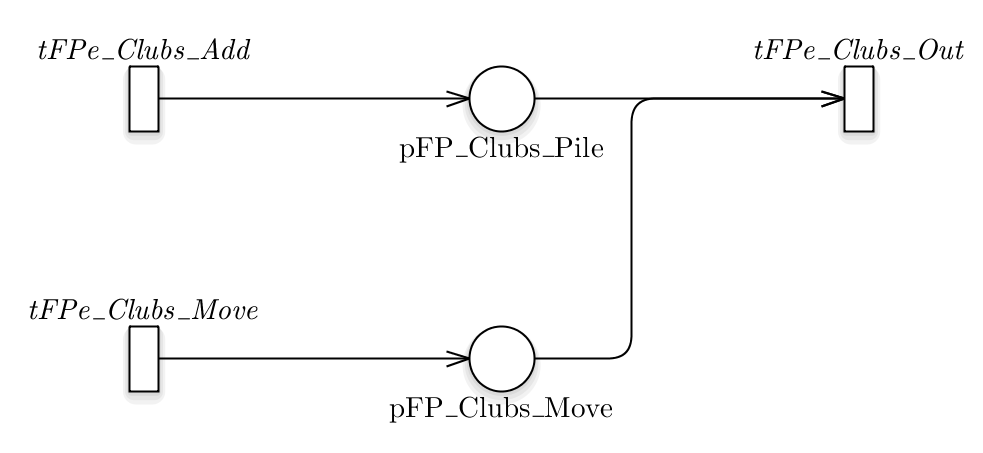
\includegraphics[width=\textwidth]{images/foundationPile}
		\caption{Foundation Pile Module}
		\label{fig:foundation_pile}
	\end{center}
\end{figure}

This module is inactive during the initial phase, and only becomes interact-able once the normal phase starts. It has two external inputs, the first of which is \verb!tFPe_Clubs_Add!. This transition has a shared pre-processor file, \verb!pre_tFPe_Add!. Listing \ref{lst:pre_tFPe_Add} shows parts of the logic, the full file can be found in \ref{app:pre_tFPe_Add}. The pre-processor fetches the token arrived earliest at \verb!pMC_Out_Buffer!. This is an important step, but is not strictly required because of the limitations the resource \verb!playerAction! enforces on the transitions of the Player and Player Bot modules. Still, it makes sense to fetch the earliest token in \ac{fifo} style to make sure that the first moved card reaches its destination first. 
\newline

Given that the colors of the token have the correct length, the \verb!get_suit_from_transname! function will be run to determine which \ac{fp} the executing transition belongs to. More information about this step can be found in \ref{sec:2_file_structure}. Lastly, the \verb!checkCommand_Move! function is ran to determine the validity of the command in the context of this particular transition. The \verb!checkCommand_Move! function is quite involved, and is discussed in detail in chapter \ref{sec:3_move_command}.
\lstinputlisting[style=matlabcode,caption=pre\_tFPe\_Add.m lines 5-17,label=lst:pre_tFPe_Add,firstline=5,lastline=17]{\GPenSIM/pre_tFPe_Add.m}

The second external input is \verb!tFPe_Clubs_Move!. Its used for moving cards to other modules, and works similarly to how movement in handle in the Draw Pile, with the additional caveat that all four Foundation Piles becomes enabled at the time from \verb!pMC_FP_Move!. Due to this its necessary to introduce additional logic to ensure that the issued move-command from the Player or Player Bot modules are meant for this particular module. As with the other modules, the actual validity of the move-command are handles by the \ac{p} and \ac{pb} modules.
\lstinputlisting[style=matlabcode,caption=pre\_tFPe\_Move.m lines 4-10,label=lst:pre_tFPe_Move,firstline=4,lastline=10]{\GPenSIM/pre_tFPe_Move.m}

The only external output of the {fp} is \verb!tFPe_Clubs_Out!. It works similarly to the output of the Draw Pile, where the pre-processor takes the latest arrived card \verb!pFP_Clubs_Pile! and the earliest arrived command from \verb!pFP_Clubs_Move!. This ensures that the first issued command will be processed first, should there be more than one. The only time there would be more than one command executing concurrently is if neither the Player or the Player Bot modules where enabled, and the command was issued from another module which did not use the \verb!playerAction! resource. Listing \ref{lst:pre_tFPe_Out} shows parts of the code.
\lstinputlisting[style=matlabcode,caption=pre\_tFPe\_Out.m lines 4-10,label=lst:pre_tFPe_Out,firstline=4,lastline=10]{\GPenSIM/pre_tFPe_Out.m}


Another interesting fact about the Foundation Pile modules is the place \verb!pFP_Clubs_Pile!. Once this place is filled with 13 tokens for all the suits, the game is won, and the simulation ends. There is no check done on the actual color or order of the tokens, as that is done when adding them by the pre-processor of \verb!tFPe_Clubs_Add!. The win condition can be found in \verb!COMMON_POST!. Parts of the code is shown in listing \ref{lst:COMMON_POST}.
\lstinputlisting[style=matlabcode,caption=COMMON\_POST.m lines 36-45,label=lst:COMMON_POST,firstline=36,lastline=45]{\GPenSIM/COMMON_POST.m}
\begin{table}
	\caption{Places and transitions used in Foundation Pile - Clubs}
	\begin{tabular}{|l|l|l|}
		\hline
		& Name & Description \\
		\hline
		1  & pFP\_Clubs\_Move        &  Buffer for move-\ac{command}s \\ \hline
		2  & pFP\_Clubs\_Pile        &  Holds the cards which are added to the Foundation Pile.\\ \hline
		3  & tFPe\_Clubs\_Add        &  External input for adding cards to the Foundation Pile.  \\ \hline
		4 & tFPe\_Clubs\_Move        &  External input for the move-command. \\ \hline
		5 & tFPe\_Clubs\_Out         &  External output  \\ \hline
	\end{tabular}
\end{table}
\clearpage
\subsection{Tableau Pile Module}
The Tableau Pile module is depicted in figure \ref{fig:tableau_pile}. It is duplicated 7 times, once for every pile in the tableau. The main difference between these modules is the names of their respective transitions and names, so the description given for the first pile will count for the other duplicates as well. Another difference is how many cards each pile are dealt during the initial phase. This is discussed in more detail in chapter \ref{sec:3_initial_dealing} and \ref{sec:draw_pile}. All the pre- and post-processor files are shared between all piles.
\begin{figure}
	\begin{center}
		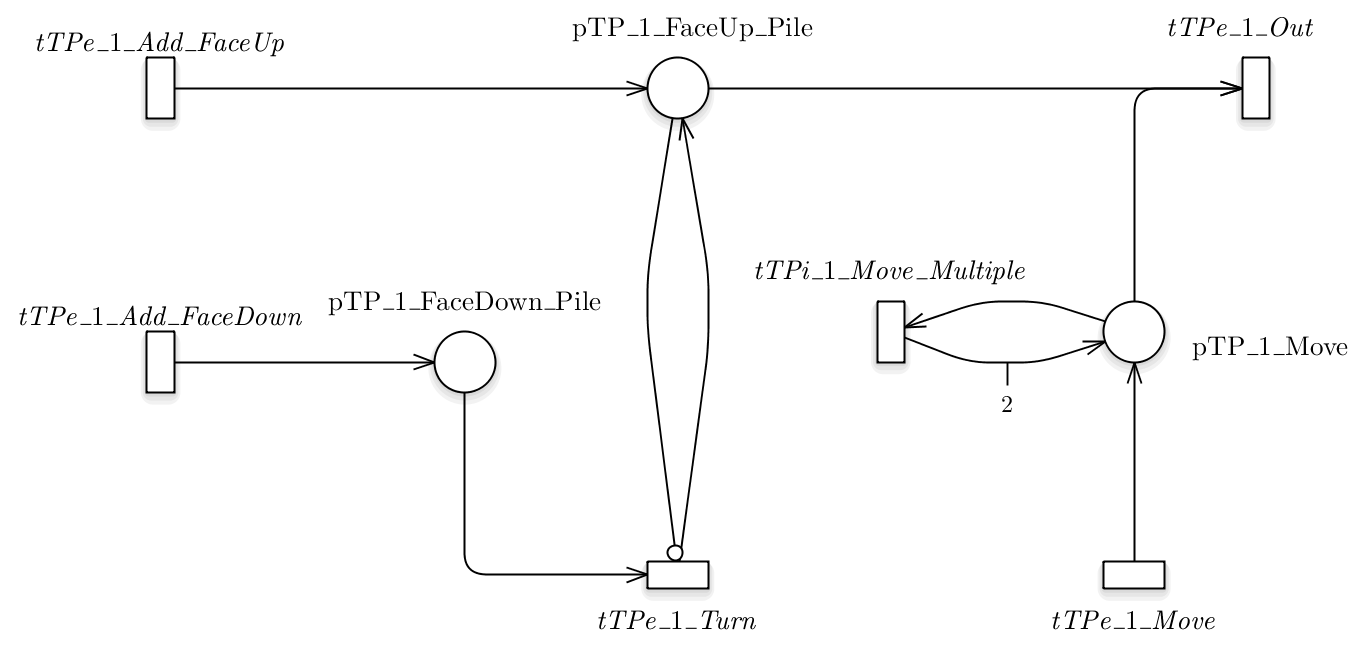
\includegraphics[width=\textwidth]{images/tableauPile}
		\caption{Tableau Pile Module}
		\label{fig:tableau_pile}
	\end{center}
\end{figure}

As with the Draw Pile module, the module encompasses both a face-down and a face-up pile. The inner workings between these two piles is different however, as moving a card from the face-down pile to the face-up pile is an non-reversible action. Doing so could put the game in an unsolvable state, but at the same time if there were no cards in any of the face-down piles the game would be trivial to solve. \\

The only time it's possible to add cards to \verb!pTP_1_FaceDown_Pile! is during the initial phase. During this phase, one less than the piles identification number will be added, so that pile one will have zero cards in the face-down pile, whilst pile 7 will have 6. All the piles will have a single card added to \verb!pTP_1_FaceUp_Pile!. This is discussed in more detail in chapter \ref{sec:3_initial_dealing}. \\

Once the initial phase is over, the pre-processor of \verb!tTPe_1_Add_FaceDown! will prevent any more firings. This is shown in listing \ref{lst:pre_tTPe_Add_FaceDown}, and is done by simply counting how many cards have been dealt in the variable \verb!global_info.CARDS.DEALT!. The secondary condition in the if statement is used to control the amount of firings during the initial phase.
\lstinputlisting[style=matlabcode,caption=pre\_tTPe\_Add\_FaceDown.m lines 5-11,label=lst:pre_tTPe_Add_FaceDown,firstline=5,lastline=11]{\GPenSIM/pre_tTPe_Add_FaceDown.m}

Instead, the \verb!tTPe_1_Add_FaceUp! transition will have potential to fire, given that all of its conditions in the pre-processor is fulfilled. Parts of the code for the pre-processor can be found in listing \ref{lst:pre_tTPe_Add_FaceUp}, whilst the whole file is found in \ref{app:pre_tTPe_Add_FaceUp}. The main job of the pre-processor is to check whether the game is still in the initial phase, and if so, how many cards have been added to \verb!pTP_1_FaceDown_Pile!. While the game is in the initial phase, there are no checks on the the suit or rank of the cards being added, but once it enters the normal phase, the pre-processor will rely on the \verb!checkCommand_Move! function to check the validity against the actual Solitaire rules. More information about the \verb!checkCommand_Move! function is found in chapter \ref{sec:3_move_command}. 
\lstinputlisting[style=matlabcode,caption=pre\_tTPe\_Add\_FaceUp.m lines 7-31,label=lst:pre_tTPe_Add_FaceUp,firstline=7,lastline=31]{\GPenSIM/pre_tTPe_Add_FaceUp.m}

Both the \verb!tTPe_1_Add_FaceDown! and \verb!tTPe_1_Add_FaceUp! also have post-processors which will increment the variable \verb!global_info.CARDS_DEALT!. The post-processor for \verb!tTPe_1_Add_FaceUp! also decrements the variable \\\verb!global_info.TP_Move_Multiple_Count! which is used when multiple cards are to be moved from the pile. Listing \ref{lst:post_tTPe_Add_FaceUp} shows how the variable is decremented, and once the last card has been received, the \verb!playerAction! resource will be released. Full code for the post-processor can be found in \ref{app:post_tTPe_Add_FaceUp}. More details on moving multiple cards will follow in the next paragraphs.
\lstinputlisting[style=matlabcode,caption=post\_tTPe\_Add\_FaceUp.m lines 5-12,label=lst:post_tTPe_Add_FaceUp,firstline=5,lastline=12]{\GPenSIM/post_tTPe_Add_FaceUp.m}

The module encompasses two external inputs, there first of which is \verb!tTPe_1_Turn!. As can be seen in figure \ref{fig:tableau_pile}, the transition is only enabled if there is at least one token in \verb!pTP_1_FaceDown_Pile! and no tokens in \verb!pTP_1_FaceUp_Pile!. The transitions pre-processor will check that the command in \verb!pMC_TP_Turn! is meant for this particular pile. This is done through extracting the unique identifier using the function \verb!get_tableau_from_transname!. \newline

The next external input is \verb!tTPe_1_Move!, which works similarly to the movement inputs of \ac{dp} and \ac{fp}, but with one big difference; it supports moving multiple cards at a time. This is achieved in conjunction with \verb!tTPi_1_Move_Multiple! using two global variables shown in listing \ref{lst:pre_tTPe_Move}. Note that it is only possible to move multiple cards to other \ac{tp}.
\lstinputlisting[style=matlabcode,caption=pre\_tTPe\_Move.m lines 11-19,label=lst:pre_tTPe_Move,firstline=11,lastline=19]{\GPenSIM/pre_tTPe_Move.m}

The same functionality could be achieved using only one variable, however by using two we make sure that the \verb!playerAction! resource remains taken until all the cards have reached their destination. When \verb!tTPi_1_Move_Multiple! fire it will take the token in \verb!pTP_1_Move!, and return two new ones, essentially duplicating the token. By doing this one time less than the amount of cards to be moved, we end up with the desired number of tokens in \verb!pTP_1_Move!. Listing \ref{lst:pre_tTPi_Move_Multiple} shows the pre-processor of \verb!tTPi_1_Move_Multiple!, and listing \ref{lst:COMMON_POST_2} shows how \verb!global_info.TP_Move_Multi_Gen_Tokens! is decremented in the \verb!COMMON_POST! file.
\lstinputlisting[style=matlabcode,caption=pre\_tTPi\_Move\_Multiple.m lines 6-13,label=lst:pre_tTPi_Move_Multiple,firstline=6,lastline=13]{\GPenSIM/pre_tTPi_Move_Multiple.m}

\lstinputlisting[style=matlabcode,caption=COMMON\_POST.m lines 28-34,label=lst:COMMON_POST_2,firstline=28,lastline=34]{\GPenSIM/COMMON_POST.m}

The only external output is \verb!tTPe_1_Out!, which will only fire once enough tokens are generated by \verb!tTPi_1_Move_Multiple!. In order ensure that the correct card is moved, the pre-processor will fetch the \textbf{n}-th latest arrived card. Where \textbf{n} is the number of tokens in \verb!pTP_1_Move!. This is repeated for every token in \verb!pTP_1_Move!. By doing this, correctness is preserved by always moving the highest ranking card first. Listing \ref{lst:pre_tTPe_Out} shows the main logic of the pre-processor, the whole file is found in at \ref{app:pre_tTPe_Out}.
\lstinputlisting[style=matlabcode,caption=pre\_tTPe\_Out.m lines 6-19,label=lst:pre_tTPe_Out,firstline=6,lastline=19]{\GPenSIM/pre_tTPe_Out.m}

\begin{table}
	\caption{Places and transitions used in Tableau Pile - 1}
	\begin{tabular}{|l|l|l|}
		\hline
		& Name & Description \\
		\hline
		1 & pTP\_1\_FaceDown\_Pile    &  Holds the face-down cards. These are not visible to the player.\\ \hline
		2 & pTP\_1\_FaceUp\_Pile      &  Holds the face-up cards. All cards are visible to the player.\\ \hline
		3 & pTP\_1\_Move              &  Buffer for move-commands\\ \hline
		4 & tTPe\_1\_Add\_FaceDown   &  External input for adding cards to the face-up pile.  \\ \hline
		5 & tTPe\_1\_Add\_FaceUp     &  External input for adding cards to the face-down pile during the initial phase.  \\ \hline
		6 & tTPe\_1\_Move            &  External input for the move-command.  \\ \hline
		7 & tTPe\_1\_Out             &  External output  \\ \hline
		8 & tTPe\_1\_Turn            &  External input for the turn-command.  \\ \hline
		9 & tTPi\_1\_Move\_Multiple  &  Internal transition which duplicates the move-command when moving multiple cards.  \\ \hline
	\end{tabular}
\end{table}
\clearpage
\subsection{Player Module}
The Player module is a set of 20 transitions, tightly knit with the \ac{gui} and the Module Connector. This module differs from the \ac{dp}, \ac{fp} and \ac{tp} modules in that the arcs to the Module Connector are done in the Player module rather than in the Module Connector. By doing this, it is possible to toggle this module on/off in the variable \verb!global_info.GUI_ENABLED!.
\begin{figure}
	\begin{center}
		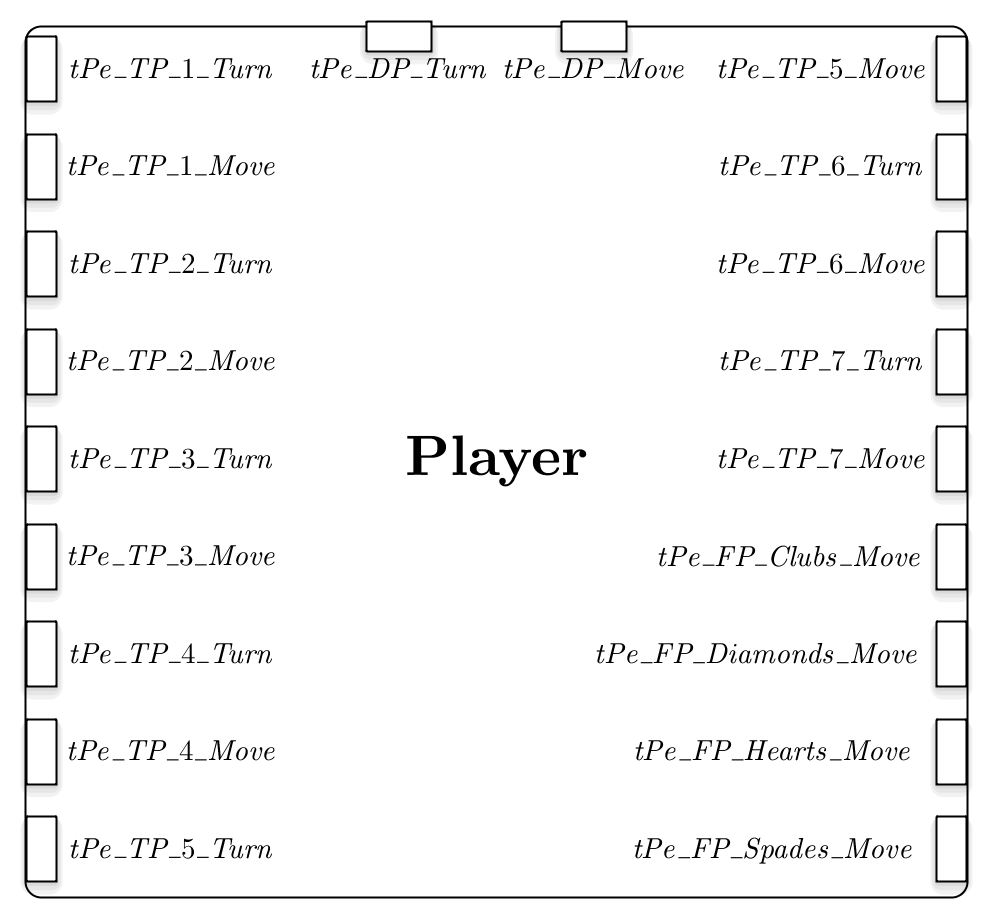
\includegraphics[scale=0.6]{images/playerModule}
		\caption{Player module}
		\label{fig:player_module}
	\end{center}
\end{figure}\\
An important aspect of the Player module is the acquisition of the \verb!playerAction! resource in the pre-processor file of every transition. By doing this, the atomicity of each action is preserved, as it's not possible to start a new action before the previous one finishes executing. Resources are discussed in more detail in chapter \ref{sec:3_Resources}.\\

In order to make the buttons of the GUI be responsive, it was necessary to introduce the \verb!pause! command in one of the pre-processors. For this, the \verb!tPe_DP_Turn_pre! pre-processor was chosen. It's a bit unclear what exactly happens when the \verb!pause! command executes, but I suspect Matlab has a seperate event queue for all GUI elements. This queue is likely checked every time the main program execution is halted with \verb!pause!. There might be a more elegant way of doing this, but none was located. Having the \verb!pause! command execute in the pre-processor executes might not be well-suited for real-time simulations as it might introduce bias in the timings. In this project however, this solution worked very well, with no problems or unresponsiveness at all.
\lstinputlisting[style=matlabcode,caption=tPe\_DP\_Turn\_pre.m,label=lst:tPe_DP_Turn_pre]{\GPenSIM/tPe_DP_Turn_pre.m}

As can be seen in listing \ref{lst:tPe_DP_Turn_pre}, to check if a button is pressed is actually a matter of checking whether the global variable corresponding to that button is set. In the listing above, it is accomplished by checking if \verb!global_info.DP_Turn_Btn! is set, and if so set it back to false. A consequence of doing this, is that it's possible to queue up actions, for example by hitting the \ac{dp} Turn-button when the game is in process of moving cards from one pile to another. \\

When issuing a new move command, its destination and possibly amount of cards to be moved is fetched directly from the GUI elements. This is done with the function \verb!get_handle!, which is a simple extension of \verb!get!, with the difference that GUI elements will only be fetched if \verb!global_info.GUI_ENABLED! is set to \verb!true!.
\begin{table}
	\caption{Transitions used in Player}
	\begin{tabular}{|l|l|l|}
		\hline
		& Name & Description \\
		\hline
		1 & tPe\_DP\_Move            &  Sends a move command to the DP module.  \\ \hline
		2 & tPe\_DP\_Turn            &  Sends a turn command to the DP module.  \\ \hline
		3 & tPe\_FP\_Clubs\_Move     &  Sends a move command to the FP Clubs module.  \\ \hline
		4 & tPe\_FP\_Diamonds\_Move  &  Sends a move command to the FP Diamonds module.  \\ \hline
		5 & tPe\_FP\_Hearts\_Move    &  Sends a move command to the FP Hearts module.  \\ \hline
		6 & tPe\_FP\_Spades\_Move    &  Sends a move command to the FP Spades module.  \\ \hline
		7 & tPe\_TP\_1\_Move         &  Sends a move command to the TP 1 module.  \\ \hline
		8 & tPe\_TP\_1\_Turn         &  Sends a turn command to the TP 1 module.  \\ \hline
		9 & tPe\_TP\_2\_Move         &  Sends a move command to the TP 2 module.  \\ \hline
		10 & tPe\_TP\_2\_Turn        &  Sends a turn command to the TP 2 module.  \\ \hline
		11 & tPe\_TP\_3\_Move        &  Sends a move command to the TP 3 module.  \\ \hline
		12 & tPe\_TP\_3\_Turn        &  Sends a turn command to the TP 3 module.  \\ \hline
		13 & tPe\_TP\_4\_Move        &  Sends a move command to the TP 4 module.  \\ \hline
		14 & tPe\_TP\_4\_Turn        &  Sends a turn command to the TP 4 module.  \\ \hline
		15 & tPe\_TP\_5\_Move        &  Sends a move command to the TP 5 module.  \\ \hline
		16 & tPe\_TP\_5\_Turn        &  Sends a turn command to the TP 5 module.  \\ \hline
		17 & tPe\_TP\_6\_Move        &  Sends a move command to the TP 6 module.  \\ \hline
		18 & tPe\_TP\_6\_Turn        &  Sends a turn command to the TP 6 module.  \\ \hline
		19 & tPe\_TP\_7\_Move        &  Sends a move command to the TP 7 module.  \\ \hline
		20 & tPe\_TP\_7\_Turn        &  Sends a turn command to the TP 7 module.  \\ \hline
	\end{tabular}
\end{table}
\clearpage
\subsection{Player Bot Module}
As with the Player module, the connections to the Module Connector is done within this module. This makes it possible to toggle this module on/off with the variable \verb!global_info.BOT_ENABLED!. The module is depicted in figure \ref{fig:player_bot_module}. In earlier iterations of the module it also had an additional place before \verb!tPBi_Gen!, an arc going from \verb!tPBi_Gen! to this place and a transition connected to this place. This worked fine, however it was found desirable to be able to toggle the bot on/off when doing testing and/or analysis. Therefore these where removed, and \verb!tPBi_Gen! simply serves as a generator when its conditions in the pre-processor are met.
\begin{figure}
	\begin{center}
		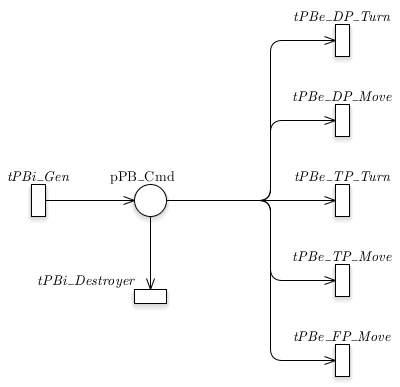
\includegraphics[scale=0.65]{images/playerBotModule}
		\caption{Player Bot module}
		\label{fig:player_bot_module}
	\end{center}
\end{figure}\\
In addition to the requirement of \verb!global_info.BOT_ENABLED! must be set to true, the pre-processor of \verb!tPBi_Gen! will check that there are no active actions ongoing, and that the previously executed command has exhausted all its parameters. To check whether there are any actions currently ongoing, the global \verb!PN! structure is checked. In this structure, all resources and their current usage can be found. Since the model only uses a single resource, it's enough to check if the first resource is taken by any transition. Listing \ref{lst:tPBi_Gen_pre} shows how this is done by calling \verb!PN.system resources.instance usage(1,1)!.

\lstinputlisting[style=matlabcode,caption=tPBi\_Gen\_pre.m lines 9-28,label=lst:tPBi_Gen_pre,firstline=9,lastline=28]{\GPenSIM/tPBi_Gen_pre.m}
The listing above also shows parts of how the module generates the commands. As this project is not really focused on AI programming, the logic for generating commands is very simple and serves more as a proof of concept. The bot possesses no ability to view the state of the game before making a decision about which command is most appropriate, rather it will simply pick a random number between 1 and 100, and select the command according to the distribution found in \verb!global_info.BOT_ACTIONS!. Listing \ref{lst:main_simulation_file} shows the three variables which control the distribution of the bots actions. 
\lstinputlisting[style=matlabcode,caption=main\_simulation\_file.m lines 19-29,label=lst:main_simulation_file,firstline=19,lastline=29]{\GPenSIM/main_simulation_file.m}

\verb!global_info.BOT_ACTIONS! is a row vector with 4 elements numbered from 1 to 100. The bot has 5 possible commands; \verb!DP_Turn!, \verb!DP_Move!, \verb!FP_Move!, \verb!TP_Turn!, and \verb!TP_Move!. Given a random numbers generated from 1-100, the probability distribution for the commands is as follows; \verb!DP_Turn! between 1 and the first element of the vector, \verb!DP_Turn! between the first and second element, \verb!FP_Move! between the second and third element, \verb!TP_Turn! between the third and fourth element, and \verb!TP_Move! between the forth element and 100.
\verb!global_info.BOT_ACTIONS_TP_TP! defines how often (on average) the bot will attempt to move a card from a \ac{tp} pile to another \ac{tp} pile versus a \ac{fp} pile. Listing \ref{lst:main_simulation_file} shows this value set to 15, which means that the bot will opt to move to another \ac{tp} pile only 15 percent of the time.\\
Finally, the \verb!global_info.BOT_ACTIONS_TP_FULL_PARTIAL_MOVE! works in a similar way, as it defines how often the \ac{tp} pile will attempt to move all the cards in the face-up pile versus just a subset of them.\\
By manipulation these values, the likelihood of solving the game will be drastically altered. Of course having a smarter bot which took actions after considering the game state, and perhaps learned from its mistake would be must better. However, this was outside the scope of this project. Future work is discussed in more detail in chapter \ref{sec5_future_work}.
\\

Given that the bot continuously generates commands, even though they might be invalid for the current state of the game, I added the \ac{destroyer} \verb!tPBi_Destroyer!. This is transition is not strictly necessary for the model to work, but was still deemed advantageous to keep the number of active tokens in the Petri Net as low as possible. Also it makes \verb!pPB_Cmd! \textbf{safe}. Listing \ref{lst:tPBi_Destroyer_pre} shows parts of the code for the \ac{destroyer}.
\lstinputlisting[style=matlabcode,caption=tPBi\_Destroyer\_pre.m lines 3-9,label=lst:tPBi_Destroyer_pre,firstline=3,lastline=9]{\GPenSIM/tPBi_Destroyer_pre.m}


The external outputs all have pre-processors which will make them fire only if the token in \verb!pPB_Cmd! has the correct color. In addition, some pre-processors have additional logic which makes them exhaust the different movement parameters before attempting a new command. An example of this can be seen in listing \ref{lst:tPBe_DP_Move_pre}, where \verb!global_info.BOT_ACTIONS_NEW_CMD! is set to 1 once there is no more piles to attempt to move to. \verb!global_info.BOT_ACTIONS_NEW_CMD! is also set to 1 in the post-processor, if the command is successfully issued.
\lstinputlisting[style=matlabcode,caption=tPBe\_DP\_Move\_pre.m lines 16-29,label=lst:tPBe_DP_Move_pre,firstline=16,lastline=29]{\GPenSIM/tPBe_DP_Move_pre.m}
\lstinputlisting[style=matlabcode,caption=COMMON\_POST.m lines 24-27,label=lst:COMMON_POST_3,firstline=24,lastline=27]{\GPenSIM/COMMON_POST.m}
\begin{table}
	\caption{Places and transitions used in Player Bot}
	\begin{tabular}{|l|l|l|}
		\hline
		& Name & Description \\
		\hline
		1 & pPB\_Cmd          & Holds the next command to be executed. \\ \hline
		2 & tPBe\_DP\_Move    & Will fetch tokens with color: DP\_Move\\ \hline
		3 & tPBe\_DP\_Turn    & Will fetch tokens with color: DP\_Turn\\ \hline
		4 & tPBe\_FP\_Move    & Will fetch tokens with color that contains: FP\_Move \\ \hline
		5 & tPBe\_TP\_Move    & Will fetch tokens with color that contains: TP\_Move \\ \hline
		6 & tPBe\_TP\_Turn    & Will fetch tokens with color that contains: TP\_Turn \\ \hline
		7 & tPBi\_Gen         & Issues new commands once the conditions of the pre-processor are met. \\ \hline
		8 & tPBi\_Destroyer   & Makes sure at most 1 token is present at \verb!pPB_Cmd! at all times. \\ \hline
	\end{tabular}
\end{table}
\clearpage
\subsection{Module Connector}
The module connector is what makes all the different modules communicate. A figure of the module connector can be seen in figure \ref{fig:full_horizontal} or for a full vertical view, in chapter \ref{app:full_vertical} in the appendix.\\

By having all the external inputs and output of every module be only transitions, we achieve a clean-cut interface. This also makes testing each individual modules easier, as the desired colored input can be programmed in the pre-processor during testing. 
\\

The only pre- og post-processors of the module connector can be found in the \ac{destroyer} transitions. These are not strictly necessary in the current form of the model, as the Player and Player Bot modules do a good job of keep tokens with incorrect colors out. However, it might be a good idea for future work to remove this responsibility from non-essential modules. Listing \ref{lst:tMC_FP_Move_Destroyer_pre} shows the destroyer of \ac{fp} move commands.
\lstinputlisting[style=matlabcode,caption=tMC\_FP\_Move\_Destroyer\_pre.m,label=lst:tMC_FP_Move_Destroyer_pre]{\GPenSIM/tMC_FP_Move_Destroyer_pre.m}
\begin{table}
	\caption{Places and transitions used in Module Connector}
	\begin{tabular}{|l|l|l|}
		\hline
		& Name & Description \\
		\hline
		1 & pMC\_DP\_Move             & Buffer for \ac{dp} move commands. \\ \hline
		2 & pMC\_DP\_Turn             & Buffer for \ac{dp} turn commands. \\ \hline
		3 & pMC\_FP\_Move             & Buffer for \ac{fp} move commands. \\ \hline
		4 & pMC\_Out\_Buffer          & Outgoing buffer for all modules. \\ \hline
		5 & pMC\_TP\_Move             & Buffer for \ac{tp} move commands. \\ \hline
		6 & pMC\_TP\_Turn             & Buffer for \ac{tp} turn commands. \\ \hline
		7 & tMC\_DP\_Move\_Destroyer     &  Destroyer for \ac{dp} move commands. \\ \hline
		8 & tMC\_FP\_Move\_Destroyer     &  Destroyer for \ac{fp} move commands.\\ \hline
		9 & tMC\_Out\_Buffer\_Destroyer  &  Destroyer the outgoing buffer.\\ \hline
		10 & tMC\_TP\_Move\_Destroyer     &  Destroyer for \ac{tp} move commands.\\ \hline
		11 & tMC\_TP\_Turn\_Destroyer     &  Destroyer for \ac{tp} turn commands.\\ \hline
	\end{tabular}
\end{table}
\clearpage
\section{Implementation}
\label{sec:gui_init}
\subsection{\ac{gui}}
The interface developed for this project is similar to the interface of the Solitaire game.
Sorting and arranging the cards is described using the same concepts that we have defined in the Solitaire Rules section.
\begin{figure}
	\begin{center}
		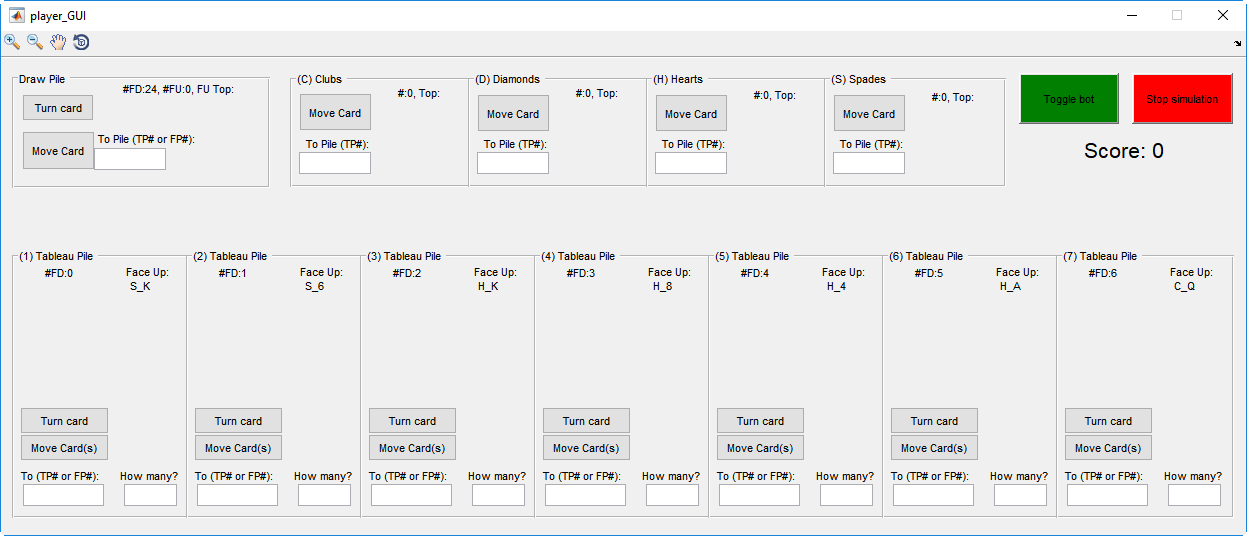
\includegraphics[width=\textwidth]{images/dealinit}
		\caption{GUI after inital dealing cards}
		\label{fig:TP4full}
	\end{center}
\end{figure}
\newline

Each pile is indexed in order to make it easier to simulate moving cards between piles. We can move cards between pile by writing the amount of cards to be moved in the "To Pile" box - see Figure \ref{fig:gui_init}.
\newline
Should the "How many?" field be left blank, only one card will be moved.
We have defined the four suits in the deck of cards:
\begin{center}
	\begin{tabular}{ | l | l | l | }
		\hline
		Suit & Cards index name \\ \hline
		Clubs & C\_A, C\_2, C\_3, C\_4, C\_5, C\_6, C\_7, C\_8, C\_9, C\_X, C\_J, C\_Q, C\_K  \\ \hline
		Diamonds & D\_A, D\_2, D\_3, D\_4, D\_5, D\_6, D\_7, D\_8, D\_9, D\_X, D\_J, D\_Q, D\_K \\ \hline
		Hearts & H\_A, H\_2, H\_3, H\_4, H\_5, H\_6, H\_7, H\_8, H\_9, H\_X, H\_J, H\_Q, H\_K  \\ \hline
		Spades & S\_A,  S\_2, S\_3,  S\_4, S\_5,  S\_6, S\_7,  S\_8, S\_9,  S\_X, S\_J, S\_Q,  S\_K \\ \hline
	\end{tabular}
\end{center}
The Index name of the card will show in the "Face Up" field for the Tableau piles, in the "FU Top" field for the Draw pile and "Top" for the foundation piles.

There are four foundation piles corresponding to the fours suits in the deck of cards:
\begin{center}
	\begin{tabular}{ | l | l | l | }
		\hline
		Index name & Pile name \\ \hline
		FPC & Foundation Pile Clubs  \\ \hline
		FPD & Foundation Pile Diamonds \\ \hline
		FPH & Foundation Pile Hearts  \\ \hline
		FPS & Foundation Pile Spades \\ \hline
	\end{tabular}
\end{center}
We have also given index names to the seven Tableau Piles:
\begin{center}
	\begin{tabular}{ | l | l | l | }
		\hline
		Index name & Pile name \\ \hline
		TP1 & Tableau Pile 1  \\ \hline
		TP2 & Tableau Pile 2 \\ \hline
		TP3 & Tableau Pile 3  \\ \hline
		TP4 & Tableau Pile 4 \\ \hline
		TP5 & Tableau Pile 5  \\ \hline
		TP6 & Tableau Pile 6  \\ \hline
		TP7 & Tableau Pile 7  \\ \hline
	\end{tabular}
\end{center}
The Draw Pile does not have an index, as we are not able to move cards back to this pile. 
The "Turn card" button allows us to shuffle to the next card in the Draw Pile. This action cannot be reversed. 
Here we can also see how many cards in the Draw Pile are facing up (\#FU), how many are facing down (\#FD) as well as the index name of the card facing up that is on top.
\newline

In accordance with the game rules that we have described in the introduction, seven of the cards are revealed initially, one on top of each tableau pile. The Draw Pile will contain 24 cards that will be revealed one at a time by clicking "Turn card".
When an Ace be revealed in the initial position of the dealt cards or by shuffling through the Draw Pile, it can be moved to its corresponding foundation pile (FP\#).
When the card that is on top of a Tableau pile is moved, the facing down card remaining on top of the pile can be turned. 
\newline
We can easily move all cards from one pile to another, as illustrated in figures \ref{fig:TP4full} and \ref{fig:TP6full}.
\begin{figure}
	\begin{center}
		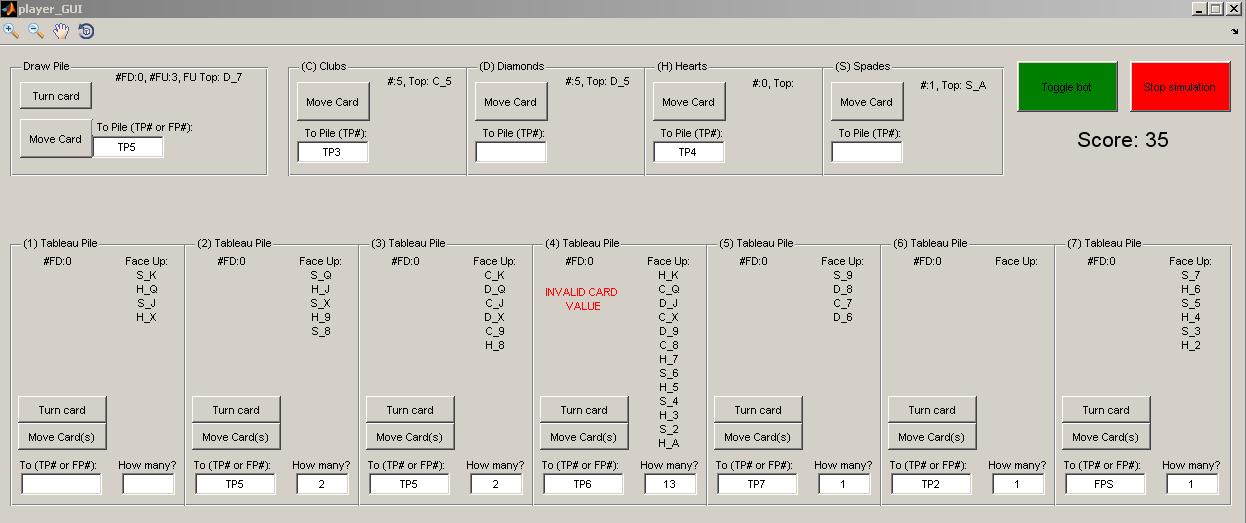
\includegraphics[width=\textwidth]{images/moveMultiple_1}
		\caption{A suite of 13 cards on Tableau pile 4 (TP4)}
		\label{fig:TP4full}
	\end{center}
\end{figure}
\begin{figure}
 	\begin{center}
 		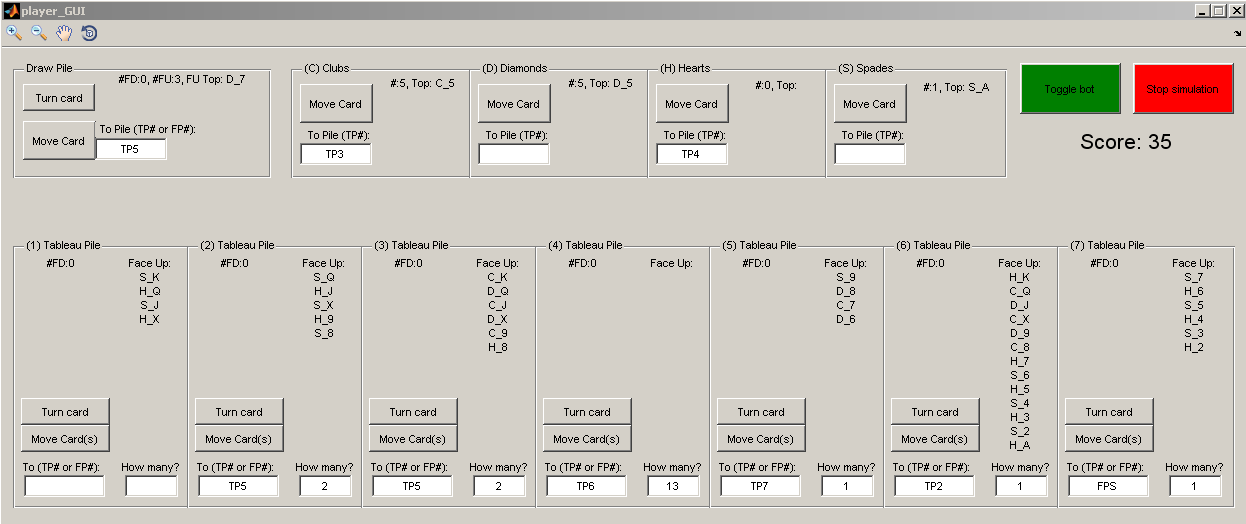
\includegraphics[width=\textwidth]{images/moveMultiple_2}
 		\caption{The cards from TP4 are moved to TP6}
 		\label{fig:TP6full}
 	\end{center}
 \end{figure}
\newline

Invalid moves such as moving a card from a different suit on the wrong foundation pile, or attempting to build down a tableau pile with two consecutve cards of the same colour are marked with the error message "Invalid move".
In the event that there are no valid moves left, the game becomes unwinnable as illustrated in figure \ref{fig:nowin}.
\begin{figure}
	\begin{center}
		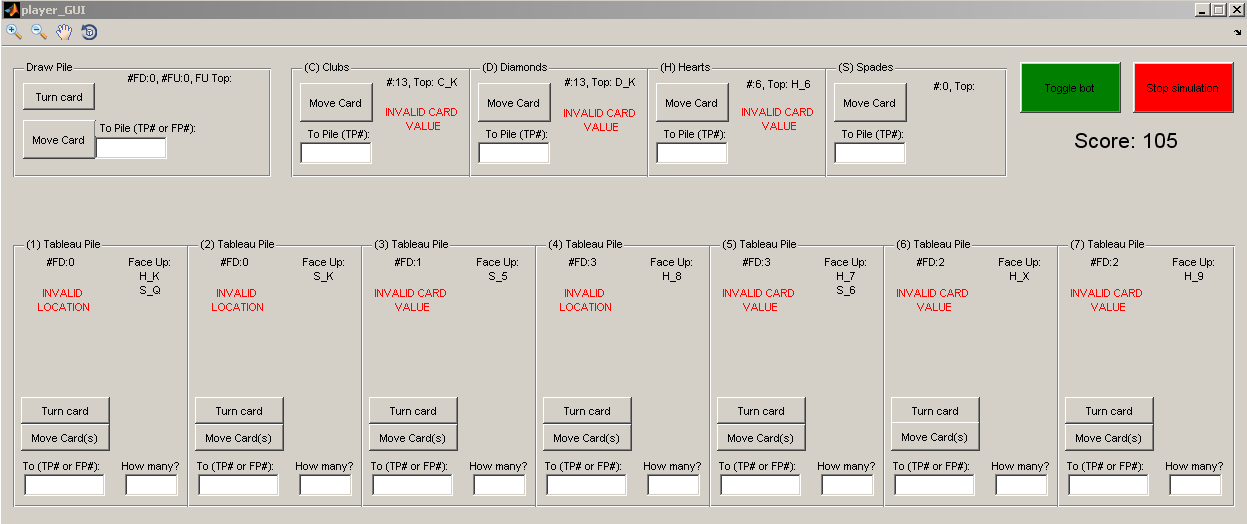
\includegraphics[width=\textwidth]{images/gameUnwinnable}
		\caption{There are no valid moves left}
		\label{fig:nowin}
	\end{center}
\end{figure}
\newline

In the event a solution is found and the foundation piles are complete, the game ends and the final amount of points displayed as shown in figure \ref{fig:win}.
\begin{figure}
	\begin{center}
		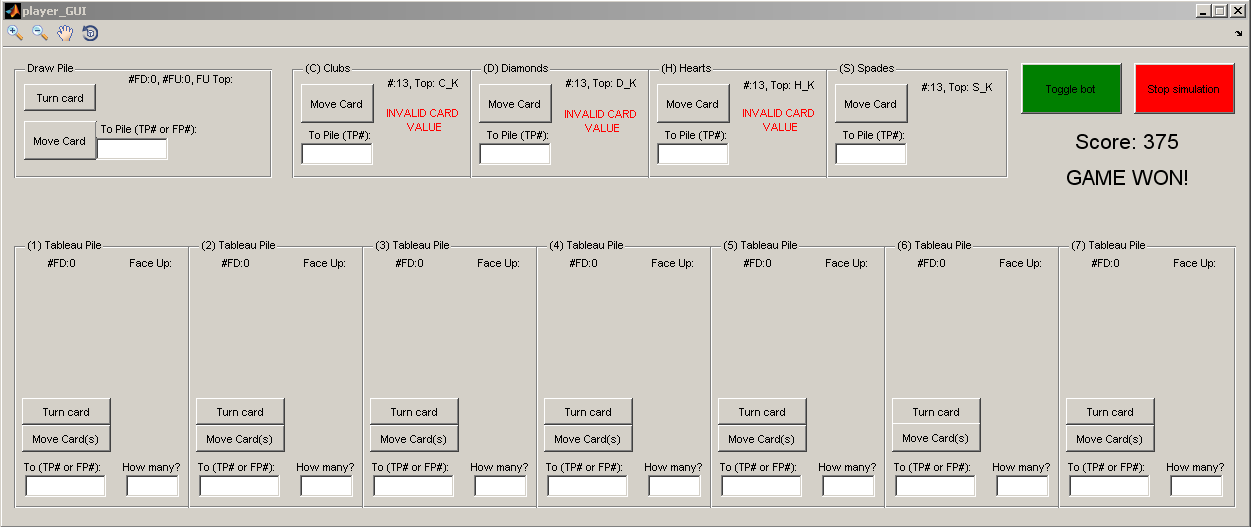
\includegraphics[width=\textwidth]{images/gameWonWScore}
		\caption{There are no valid moves left}
		\label{fig:win}
	\end{center}
\end{figure}

\label{sec:3_gui}
\clearpage
\subsection{Algorithms}
\subsubsection{Atomicity}
\clearpage
\subsection{Commands}
\subsubsection{Move Command}~\\~\\
\label{sec:3_move_command}
The move command is contains four parts; the command, destination, source and amount. Each part is concatenated together, with colon as a separator. An example of a move command would be: \textit{Move:\ac{tp}1:\ac{tp}5:3}, which means \textit{Move 3 cards from \ac{tp}1 to \ac{tp}5}. If amount is not given, it will assume one card to be moved.
\newline

In order to make sure that only validity of the move-commands, the function \verb!checkCommand_Move! has been developed. It is used both for validation before sending a command, and validation after receiving a command. The function takes the input parameters; \verb!command!, \verb!destination!, \verb!source!, and \verb!handle_err!. 
\newline

The input parameter \verb!command! contains the actual command, \verb!destination! contains the unique identifiers of the \ac{fp} or \ac{tp} modules. Valid input for \verb!destination! would be \textit{C, D, H, S, 1, 2, 3, 4, 5, 6 or 7}, and is used to ensure that the command is received by the destined module. Parameter \verb!source! is only used when sending a command, and contains the actual name of the transition which issued the game. This is mainly used to set the variable \verb!global_info.last_command_source! which will be the name of the transition holding the \verb!playerAction! resource. Resources are discussed in more detail in chapter \ref{sec:3_Resources}. Lastly, the parameter \verb!handle_err! holds the GUI-component where error mesasges will be written. Full code for the function can be found in the appendix, at chapter \ref{app:checkCommand_Move}.
\\

Figure \ref{fig:checkCommand_Move} shows a flowchart of the logic in the function.
\begin{figure}
	\begin{center}
		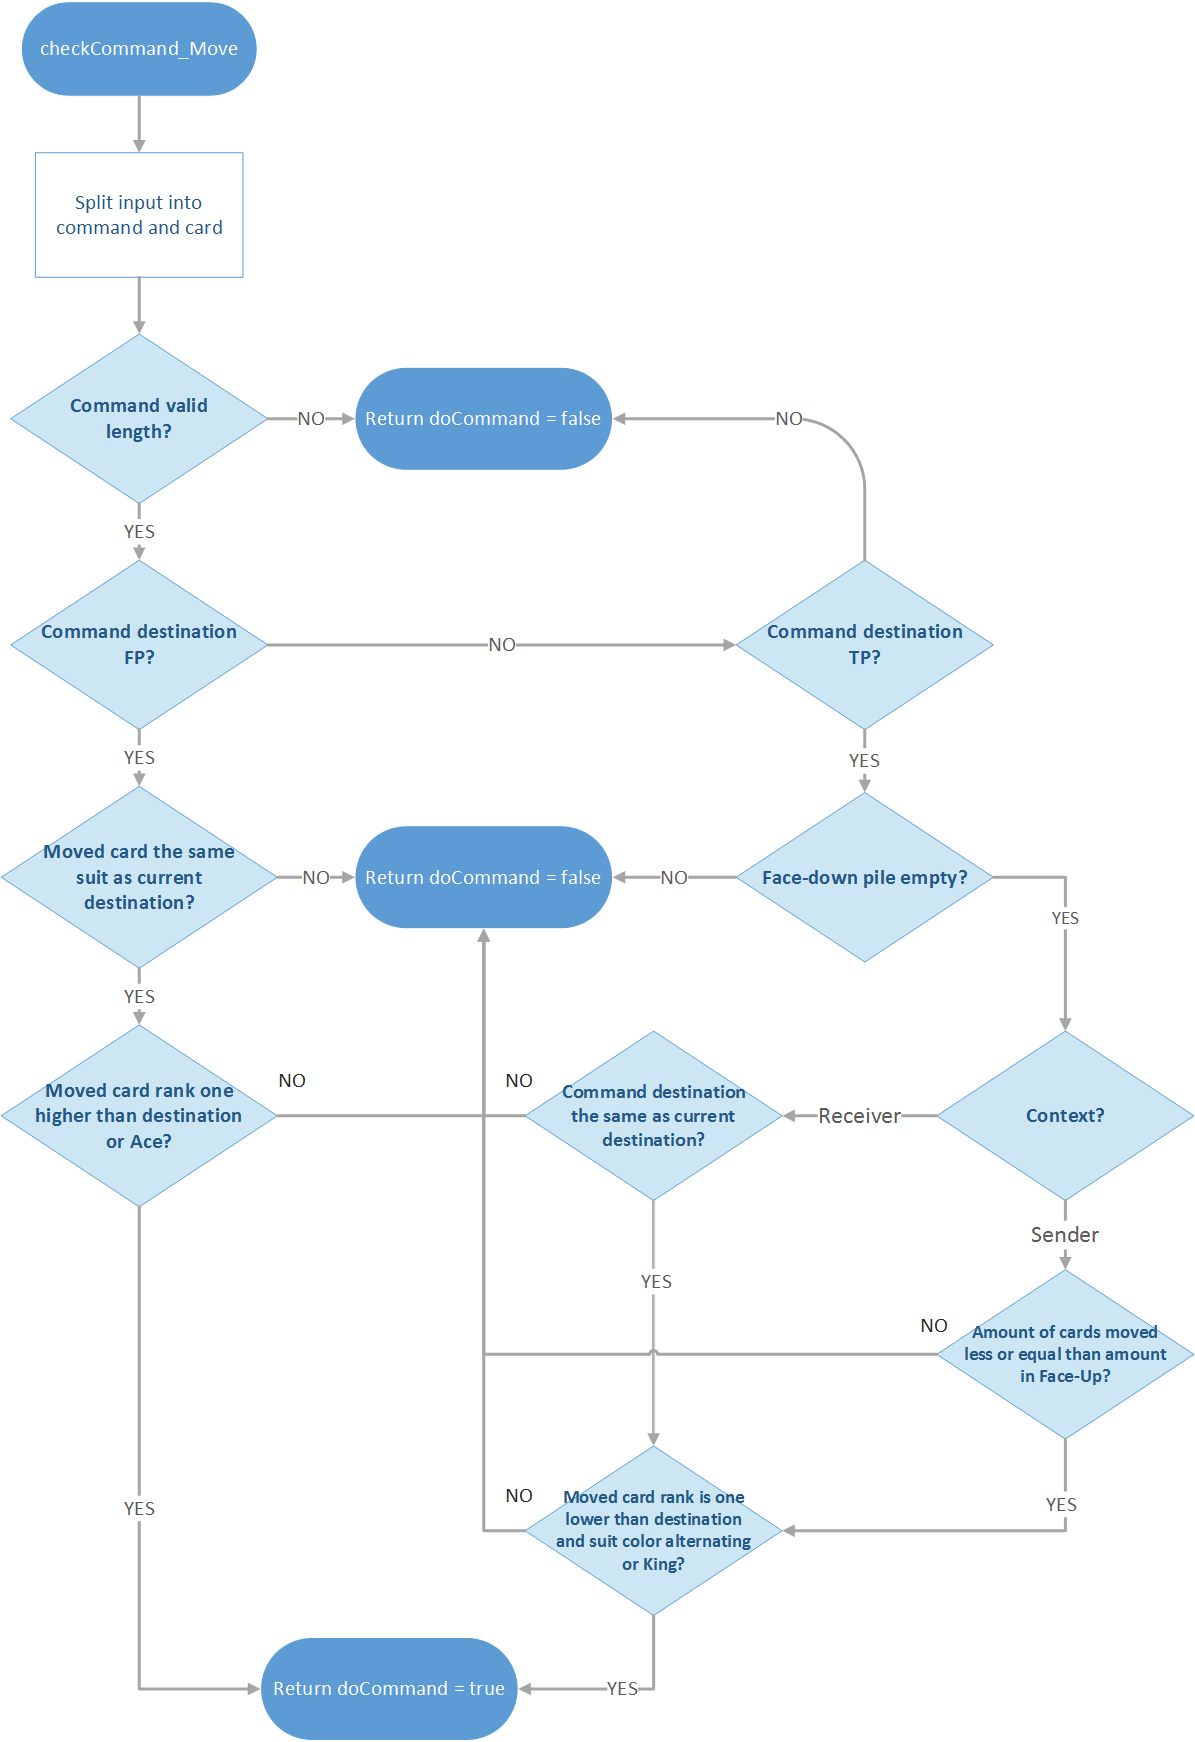
\includegraphics[width=\textwidth]{images/checkcommandmove}
		\caption{Flowchart - checkCommand\_Move}
		\label{fig:checkCommand_Move}
	\end{center}
\end{figure}
\clearpage
\subsection{Initial Dealing}
\subsection{Resources}
\label{sec:3_Resources}
The only resource used in the model is called \verb!playerAction!. It serve an essential role of the model, which is to preserve the atomicity between the different actions. To explain why this is so important, one can imagine King of Spades is about to be moved to \ac{tp}4, which is empty. Only moments later, the command to move King of Hearts is also issued to be moved to \ac{tp}4. Now, since the second move command was issued before the first card was able to reach \ac{tp}4, it will pass the validity checks, and ultimately putting the game in a completely illegal state.\\

The resource is acquired by requesting it every time either the Player or Player Bot attempts to issue a new command. If the resource is given, the name of the transition which owns it is stored in \verb!global_info.last_command_source!. Then the action can execute, knowing that no other action can execute concurrently. Once the actions is complete, the resource is released in the post-processor. Listing \ref{lst:COMMON_POST_4} shows an example of the releasing of the resource.
\lstinputlisting[style=matlabcode,caption=COMMON\_POST.m lines 16-23,label=lst:COMMON_POST_4,firstline=16,lastline=23]{\GPenSIM/COMMON_POST.m}

It's worth noting that the same functionality could be achieved by simply using a semaphore.
\subsection{Moving Multiple Cards}
\subsection{Scoring}
The standard scoring scheme in the Windows Solitaire game defines the amount of points that are awarded for moving cards between piles and is described as follows:
\begin{center}
	\begin{tabular}{ | l | l | l | }
		\hline
		Move & Points \\ \hline
		Draw pile to tableau pile & 5  \\ \hline
		Draw pile to foundation pile & 10 \\ \hline
		Tableau pile to foundation pile & 10  \\ \hline
		Turn over tableau card & 5 \\ \hline
		Foundation pile to tableau pile & -15 \\ \hline
		Reset draw pile & -100 (minimum score is 0) \\ \hline
	\end{tabular}
\end{center}


\section{Testing, Analysis and Results}
\label{sec:4_testing_analysis}
\subsection{Matlab version}
The project has been developed and tested in versions R2013a and R2017a. Due to using two versions of Matlab it was necessary to only use functionality that is supported in both versions. Examples of this is using \verb!GUIDE! for developing the GUI, and omitting to use the \verb!contains! command.

\subsection{Coverability trees}
Due to large size of the model, and the amount of initial tokens in the Draw Pile, it was not possible to get a coverability tree for the whole model. By my thinking, it should be possible to by extending the \verb!cotree! function to respect pre- and post-processors. This was outside the scope of the project, so instead I ran the \verb!cotree(pni, 1, 1)! command on the \ac{dp} and \ac{tp} modules.\\

When doing this, I had to remove arcs from the external inputs, as they would just be firing perpetually. Additionally, the names of the places and transitions where too long to be displayed in the graph, so I shortened them beforehand. A table with translates the names is included in each sub-chapter.
\subsubsection{Draw Pile}~\\
\begin{center}
	\begin{figure}
		% Left, Bottom, Right, Top
		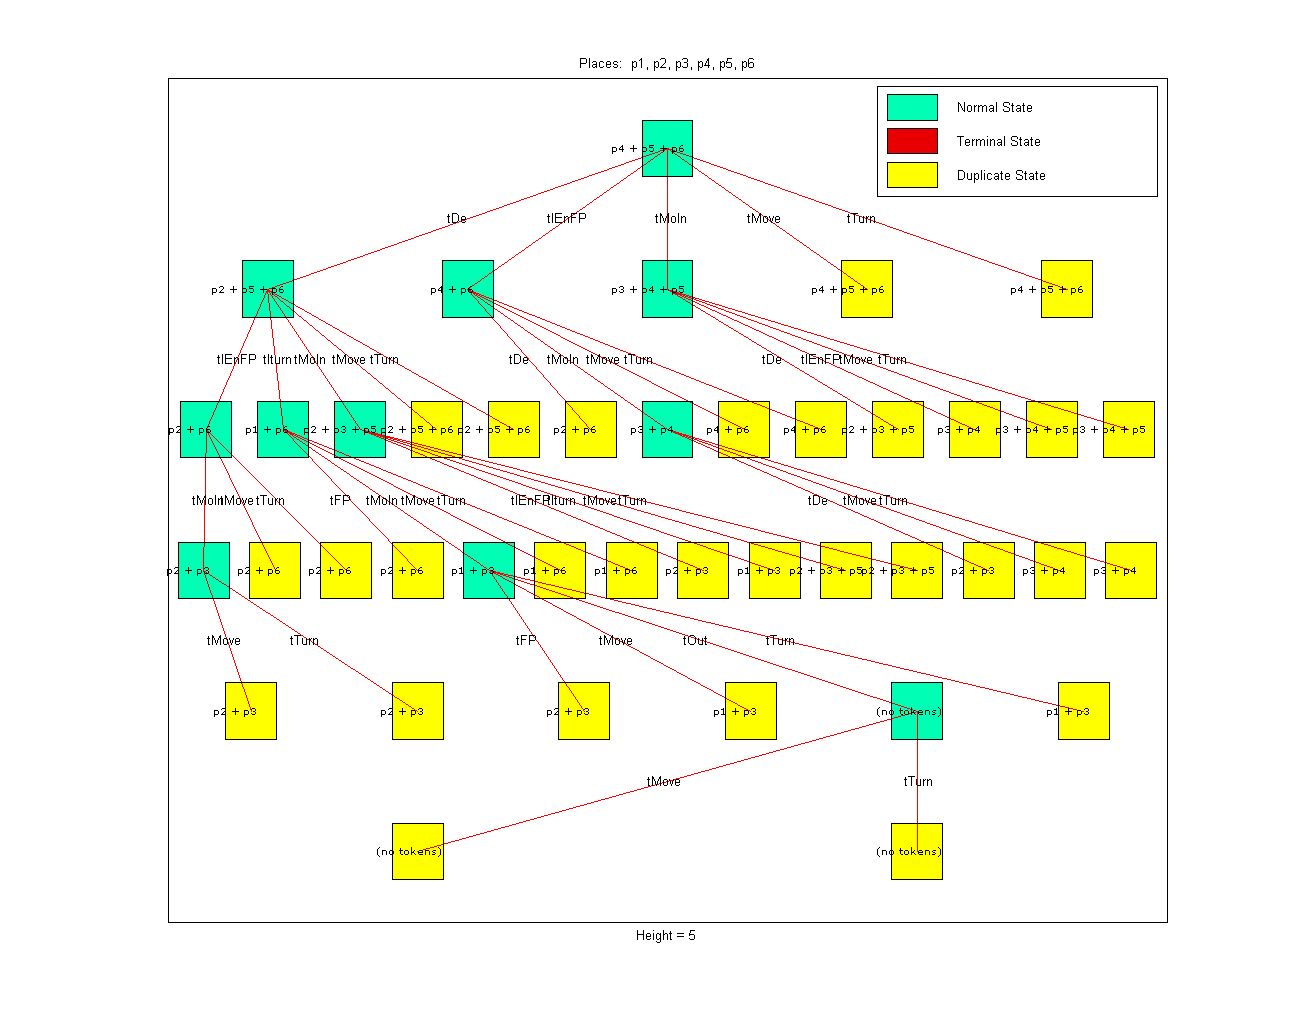
\includegraphics[trim=150 80 150 150,scale=0.5]{images/drawPile_CovTree}
		\caption{Coverability tree for Draw Pile}
		\label{fig:cov_tree_draw_pile}
	\end{figure}
\end{center}
Figure \ref{fig:cov_tree_draw_pile} shows the coverability tree generated for the Draw Pile module. 
\begin{center}
	\begin{tabular}{ | l | l | l | }
		\hline
		Name in Cov Tree & Actual name \\ \hline
		p1 & pDP\_Draw\_FaceUp\_Pile  \\ \hline
		p2 & pDP\_Draw\_FaceDown\_Pile \\ \hline
		p3 & pDP\_Move\_Out  \\ \hline
		p4 & pDP\_Dealer \\ \hline
		p5 & pDP\_Turn  \\ \hline
		p6 & pDP\_Move\_Init  \\ \hline
		tDe & tDPi\_Dealer  \\ \hline
		tOut & tDPe\_Out  \\ \hline
		tIturn & tDPi\_Turn  \\ \hline
		tIEnFP & tDPi\_Enable\_FP\_Trans  \\ \hline
		tFP & tDPi\_Flip\_Pile  \\ \hline
		tMoIn & tDPi\_Move\_Init  \\ \hline
	\end{tabular}
\end{center}
\clearpage
\subsubsection{Tableau Pile}
\begin{center}
	\begin{figure}
		% Left, Bottom, Right, Top
		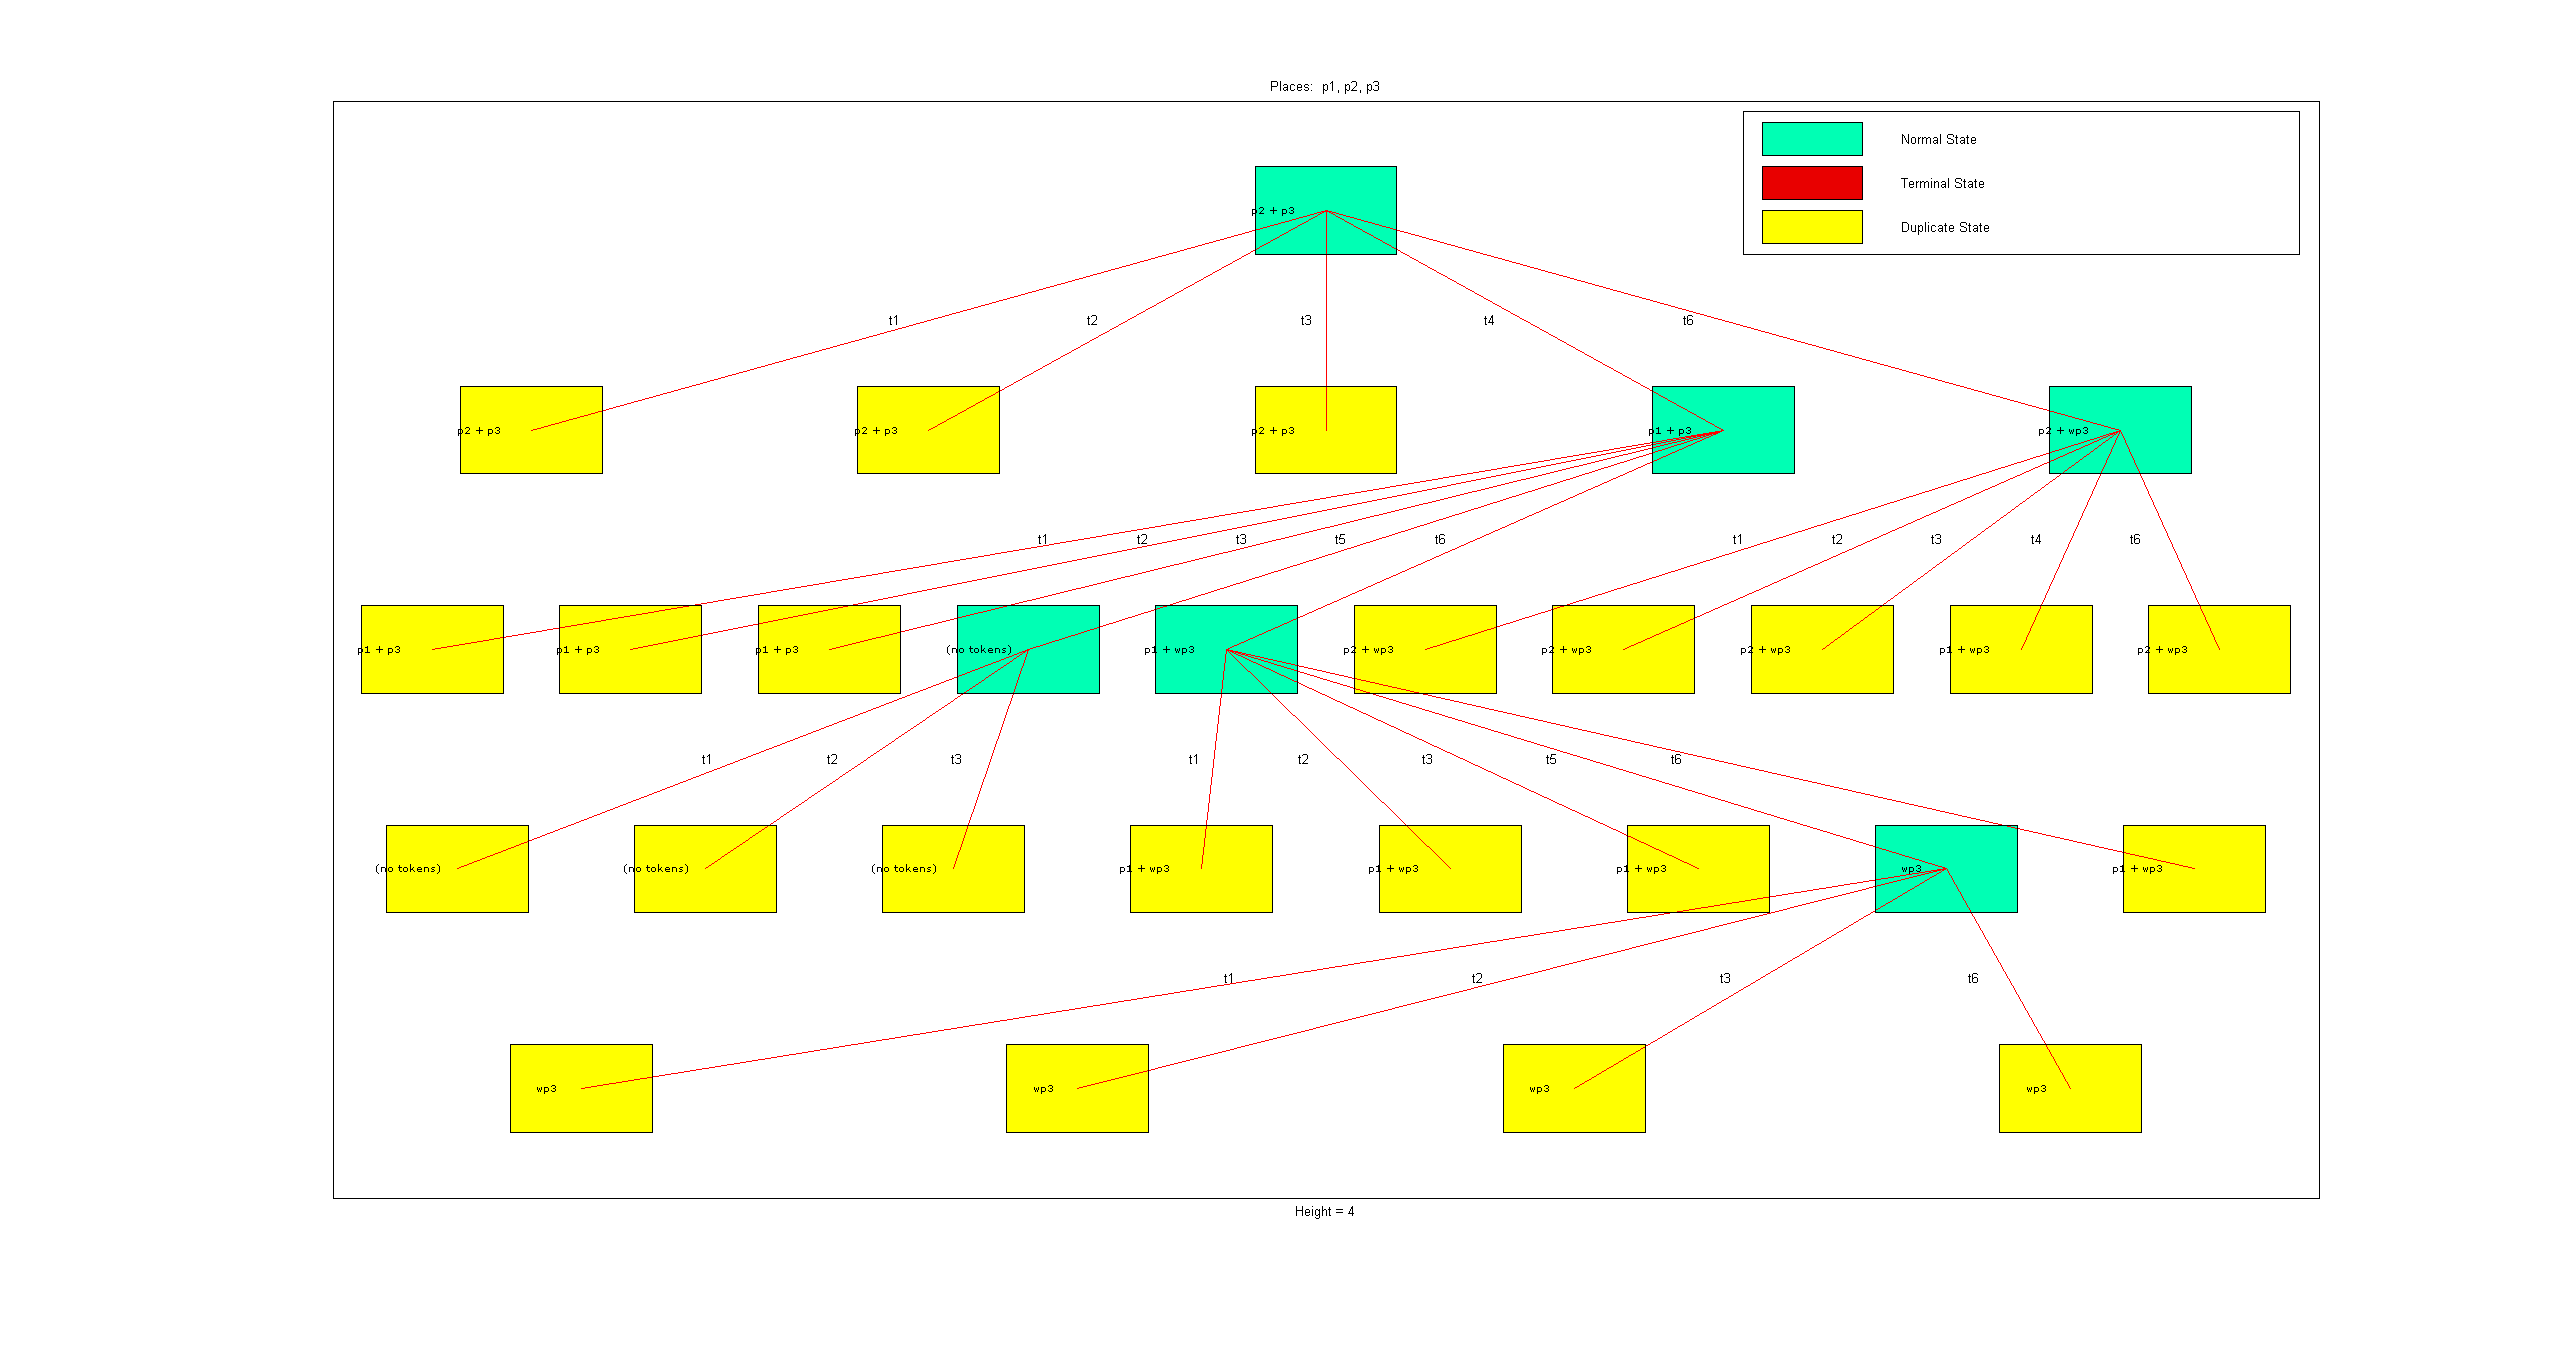
\includegraphics[trim=450 80 150 100,scale=0.3]{images/tableauPile_CovTree}
		\caption{Coverability tree for Tableau Pile}
		\label{fig:cov_tree_tableau_pile}
	\end{figure}
\end{center}
Figure \ref{fig:cov_tree_tableau_pile} shows the coverability tree generated for the Tableau Pile module. It's worth nothing that the model as a whole is k-bounded even though the cycle indicator, \textbf{w} is shown in the coverability tree. The reason for \textbf{w} is shown, is that the \verb!cotree! function does not respect the pre-processor files of the transition.
\begin{center}
	\begin{tabular}{ | l | l | l | }
		\hline
		Name in Cov Tree & Actual name \\ \hline
		p1 & pTP\_1\_FaceUp\_Pile  \\ \hline
		p2 & pTP\_1\_FaceDown\_Pile \\ \hline
		p3 & pTP\_1\_Move  \\ \hline
		t4 & tTPe\_1\_Turn  \\ \hline
		t5 & tTPe\_1\_Out  \\ \hline
		t6 & tTPi\_1\_Move\_Multiple  \\ \hline
	\end{tabular}
\end{center}
\clearpage
\subsection{Properties of the model}
\label{sec:4_properties}
\subsubsection{Boundedness}~\\
The model is k-bounded, where \textbf{k} is 52. The place with this many tokens is \verb!pDP_Dealer!, as they are initially given. Due to how the pre-processors of the Out-transitions of the modules are made, the number of tokens in any one place will never exceed 52.
\subsubsection{Liveness}~\\
The liveness of the model is limited by the siphon, \verb!pDP_Dealer!. Once the transition \verb!tDPi_Dealer! finishes firing with the initial tokens in \verb!pDP_Dealer!, it will never fire again, thus it is live at level 1. Seeing that there it is a possibility that every transition will fire, we can say that the PN is live at level 1 also.
\subsection{Structural Invariants}
\label{sec:4_structural_invariants}
\subsubsection{Siphons}~\\
\label{sec:4_siphons}
I was not able to use the built-in functionality, \verb!siphons()! to find siphons. However by analyzing the model manually, it's easy to see that the siphons of this models are: \verb!pDP_Dealer!, \verb!pTP_1__FaceDown_Pile!, \verb!pTP_2__FaceDown_Pile!, \verb!pTP_3__FaceDown_Pile!, \verb!pTP_4__FaceDown_Pile!, \verb!pTP_5__FaceDown_Pile!, \\\verb!pTP_6__FaceDown_Pile!, \verb!pTP_7__FaceDown_Pile!.
\section{Discussion}
\subsection{Originality of this work}
I was not able to find any work that resembles this project. What differs this project is that contains a complete model of a game, and also a simple \ac{gui} to go along with it.
\subsection{Limitations of the project}
\label{sec5:limitations}
A major drawback of the destroyer \verb!tMC_Out_Buffer_Destroyer! is that if it fires, the card will actually be removed from the game, and the game becomes unsolvable. This transition will fire if the move-command of the token has an invalid destination. Due to how the Player and Player Bot modules are set up, this will never happen as they will check the validity of the move command before actually issuing the command. Still, I think it would be an improvement add an additional transition to the Draw Pile module which would accept cards from \verb!tMC_Out_Buffer_Destroyer!, instead of totally discarding them.
\newline

Another improvement would be to re-factor the code base by moving more of the validity check of the commands from the Player and Player Bot modules to the destination transitions. The Player Bot modules uses roughly 200 lines of code to always issue valid commands, I think this could be drastically reduced. By doing this it would be easier to create additional modules which could interface with the game, for example a hardware-based module.
\newline

It might also be a slight improvement to combine the Add-face-up and Add-face-down transitions of the \ac{tp} modules. By doing this, it would remove the need for the Add-face-down's pre-processor to execute once the initial phase is over. However, doing so for every Tableau Pile would require 7 more transitions and 14 more places. \\

Lastly, a performance increase might be gained by reducing the number of transitions in the Player module, or at least introducing a new place and transition. This new place would serve as an input to all of the 20 transitions of the Player module, whilst the new transition would serve as an input the new place. By doing this, the number enabled transitions, and pre-processors which would have to be executed would drastically drop.

\subsection{Future work}
\label{sec5_future_work}
Unfortunately due to the model being very complex, and the project period being only 6 weeks, there was not enough time to run thorough simulations on the model. This project may be seen as preliminary work in finding the optimal game strategies of Solitaire. \\

By having the Player Bot module completely separate from the rest of the model, it should be possible to easily improving how well the bot performs. This should be done by having the bot observe the actual state of the game before issuing a command, and possible have it learn from past mistakes.

\subsection{Learning experience}
\label{sec5_learning_experience}
The main difficulty of the project was the tight time constraint. Since I was working alone on this project, this forced me to omit several improvements, which can be seen in \ref{sec5:limitations}. It also reduced the amount of time I had to run analysis on the model, as it took a lot of development and testing to make it work properly.
\clearpage
% Keeping this for reference for now %
\begin{thebibliography}{6}

\bibitem{GPenSIMguide} Reggie Davidrajuh. GPenSIM: A Tool for Modeling and Simulation of Discrete-Event Systems. 2014
\bibitem{oreilly} Tom White, Hadoop: The Definitive Guide, 2015, \emph{ISBN: 978-1-491-90163-2}
\bibitem{dockerdocs} Docker API Docs, \url{https://docs.docker.com}
\bibitem{dat630slides} Slides from DAT630, Krisztian Balog
\bibitem{dataset} Kaggle. The Enron Email Dataset. \url{https://www.kaggle.com/wcukierski/enron-email-dataset}
\bibitem{coursematerial} Data Intensive Systems Compendium, Tomasz Wiktorski et al.

\end{thebibliography}
\addtocmark{Appendix}
\appendix
\section{Overall design - Vertical view}
\label{app:full_vertical}
\begin{figure}
	% Left, Bottom, Right, Top
	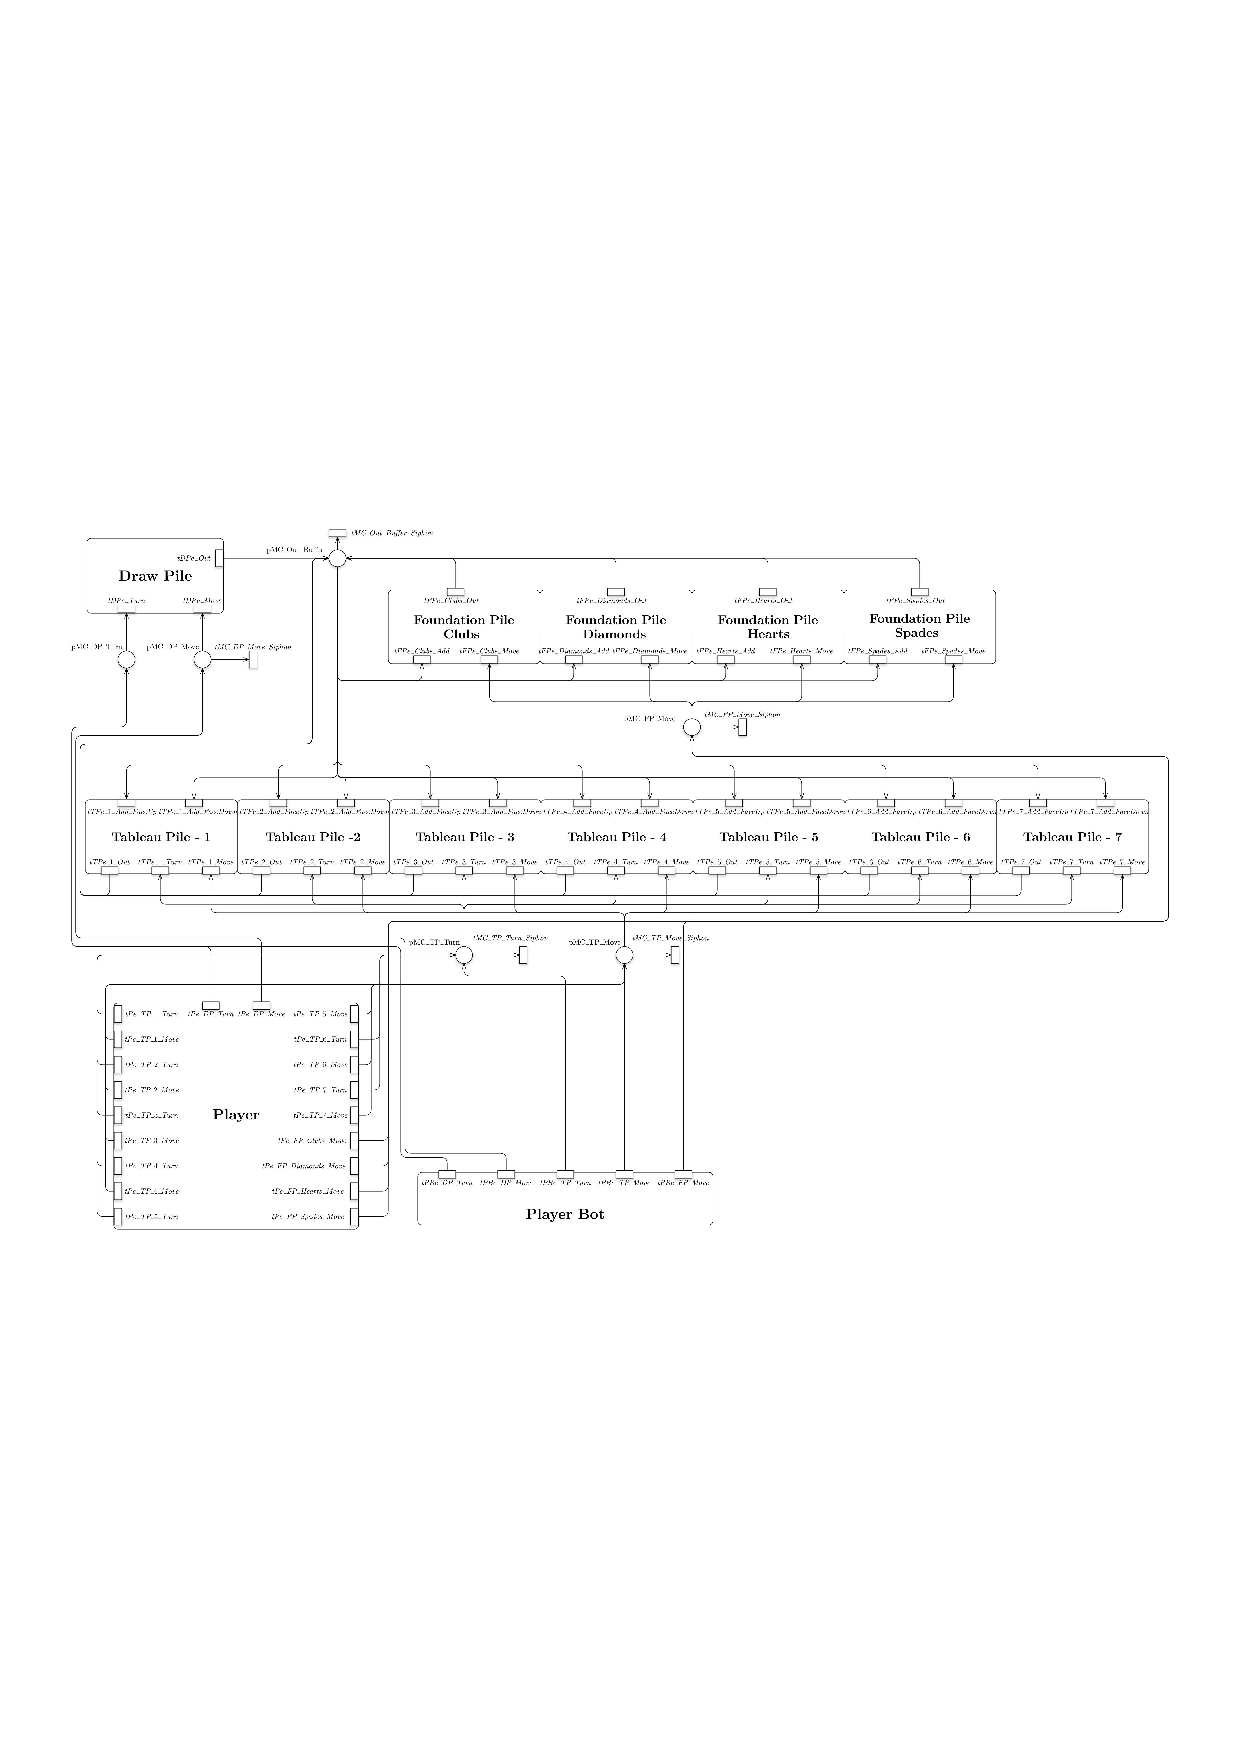
\includegraphics[trim=40 100 100 310,angle=90,scale=1.4]{images/overallViewPdf}
	\caption{The complete model in horizontal view}
	\label{fig:full_vertical}
\end{figure}
\clearpage
\section{Matlab code}	
\subsection{checkCommand\_Move.m}
\label{app:checkCommand_Move}
\lstinputlisting[style=matlabcode]{\GPenSIM/checkCommand_Move.m}

\subsection{COMMON\_POST.m}
\label{app:COMMON_POST}
\lstinputlisting[style=matlabcode]{\GPenSIM/COMMON_POST.m}

\subsection{COMMON\_PRE.m}
\label{app:COMMON_PRE}
\lstinputlisting[style=matlabcode]{\GPenSIM/COMMON_PRE.m}

\subsection{draw\_pile\_pdf.m}
\label{app:draw_pile_pdf}
\lstinputlisting[style=matlabcode]{\GPenSIM/draw_pile_pdf.m}

\subsection{foundation\_pile\_clubs\_pdf.m}
\label{app:foundation_pile_clubs_pdf}
\lstinputlisting[style=matlabcode]{\GPenSIM/foundation_pile_clubs_pdf.m}

\subsection{foundation\_pile\_diamonds\_pdf.m}
\label{app:foundation_pile_diamonds_pdf}
\lstinputlisting[style=matlabcode]{\GPenSIM/foundation_pile_diamonds_pdf.m}

\subsection{foundation\_pile\_hearts\_pdf.m}
\label{app:foundation_pile_hearts_pdf}
\lstinputlisting[style=matlabcode]{\GPenSIM/foundation_pile_hearts_pdf.m}

\subsection{foundation\_pile\_spades\_pdf.m}
\label{app:foundation_pile_spades_pdf}
\lstinputlisting[style=matlabcode]{\GPenSIM/foundation_pile_spades_pdf.m}

\subsection{get\_handle.m}
\label{app:get_handle}
\lstinputlisting[style=matlabcode]{\GPenSIM/get_handle.m}

\subsection{get\_suit\_from\_transname.m}
\label{app:get_suit_from_transname}
\lstinputlisting[style=matlabcode]{\GPenSIM/get_suit_from_transname.m}

\subsection{get\_tableau\_from\_transname.m}
\label{app:get_tableau_from_transname}
\lstinputlisting[style=matlabcode]{\GPenSIM/get_tableau_from_transname.m}

\subsection{main\_simulation\_file.m}
\label{app:main_simulation_file}
\lstinputlisting[style=matlabcode]{\GPenSIM/main_simulation_file.m}

\subsection{module\_connector\_pdf.m}
\label{app:module_connector_pdf}
\lstinputlisting[style=matlabcode]{\GPenSIM/module_connector_pdf.m}

\subsection{player\_bot\_pdf.m}
\label{app:player_bot_pdf}
\lstinputlisting[style=matlabcode]{\GPenSIM/player_bot_pdf.m}

\subsection{player\_GUI.m}
\label{app:player_GUI}
\lstinputlisting[style=matlabcode]{\GPenSIM/player_GUI.m}

\subsection{player\_pdf.m}
\label{app:player_pdf}
\lstinputlisting[style=matlabcode]{\GPenSIM/player_pdf.m}

\subsection{player\_update\_GUI.m}
\label{app:player_update_GUI}
\lstinputlisting[style=matlabcode]{\GPenSIM/player_update_GUI.m}

\subsection{post\_tTPe\_Add\_FaceUp.m}
\label{app:post_tTPe_Add_FaceUp}
\lstinputlisting[style=matlabcode]{\GPenSIM/post_tTPe_Add_FaceUp.m}

\subsection{pre\_tFPe\_Add.m}
\label{app:pre_tFPe_Add}
\lstinputlisting[style=matlabcode]{\GPenSIM/pre_tFPe_Add.m}

\subsection{pre\_tFPe\_Move.m}
\label{app:pre_tFPe_Move}
\lstinputlisting[style=matlabcode]{\GPenSIM/pre_tFPe_Move.m}

\subsection{pre\_tFPe\_Out.m}
\label{app:pre_tFPe_Out}
\lstinputlisting[style=matlabcode]{\GPenSIM/pre_tFPe_Out.m}

\subsection{pre\_tPe\_FP\_Move.m}
\label{app:pre_tPe_FP_Move}
\lstinputlisting[style=matlabcode]{\GPenSIM/pre_tPe_FP_Move.m}

\subsection{pre\_tPe\_TP\_Move.m}
\label{app:pre_tPe_TP_Move}
\lstinputlisting[style=matlabcode]{\GPenSIM/pre_tPe_TP_Move.m}

\subsection{pre\_tPe\_TP\_Turn.m}
\label{app:pre_tPe_TP_Turn}
\lstinputlisting[style=matlabcode]{\GPenSIM/pre_tPe_TP_Turn.m}

\subsection{pre\_tTPe\_Add\_FaceDown.m}
\label{app:pre_tTPe_Add_FaceDown}
\lstinputlisting[style=matlabcode]{\GPenSIM/pre_tTPe_Add_FaceDown.m}

\subsection{pre\_tTPe\_Add\_FaceUp.m}
\label{app:pre_tTPe_Add_FaceUp}
\lstinputlisting[style=matlabcode]{\GPenSIM/pre_tTPe_Add_FaceUp.m}

\subsection{pre\_tTPe\_Move.m}
\label{app:pre_tTPe_Move}
\lstinputlisting[style=matlabcode]{\GPenSIM/pre_tTPe_Move.m}

\subsection{pre\_tTPe\_Out.m}
\label{app:pre_tTPe_Out}
\lstinputlisting[style=matlabcode]{\GPenSIM/pre_tTPe_Out.m}

\subsection{pre\_tTPe\_Turn.m}
\label{app:pre_tTPe_Turn}
\lstinputlisting[style=matlabcode]{\GPenSIM/pre_tTPe_Turn.m}

\subsection{pre\_tTPi\_Move\_Multiple.m}
\label{app:pre_tTPi_Move_Multiple}
\lstinputlisting[style=matlabcode]{\GPenSIM/pre_tTPi_Move_Multiple.m}

\subsection{set\_handle.m}
\label{app:set_handle}
\lstinputlisting[style=matlabcode]{\GPenSIM/set_handle.m}

\subsection{splitCommand.m}
\label{app:splitCommand}
\lstinputlisting[style=matlabcode]{\GPenSIM/splitCommand.m}

\subsection{tableau\_pile\_1\_pdf.m}
\label{app:tableau_pile_1_pdf}
\lstinputlisting[style=matlabcode]{\GPenSIM/tableau_pile_1_pdf.m}

\subsection{tableau\_pile\_2\_pdf.m}
\label{app:tableau_pile_2_pdf}
\lstinputlisting[style=matlabcode]{\GPenSIM/tableau_pile_2_pdf.m}

\subsection{tableau\_pile\_3\_pdf.m}
\label{app:tableau_pile_3_pdf}
\lstinputlisting[style=matlabcode]{\GPenSIM/tableau_pile_3_pdf.m}

\subsection{tableau\_pile\_4\_pdf.m}
\label{app:tableau_pile_4_pdf}
\lstinputlisting[style=matlabcode]{\GPenSIM/tableau_pile_4_pdf.m}

\subsection{tableau\_pile\_5\_pdf.m}
\label{app:tableau_pile_5_pdf}
\lstinputlisting[style=matlabcode]{\GPenSIM/tableau_pile_5_pdf.m}

\subsection{tableau\_pile\_6\_pdf.m}
\label{app:tableau_pile_6_pdf}
\lstinputlisting[style=matlabcode]{\GPenSIM/tableau_pile_6_pdf.m}

\subsection{tableau\_pile\_7\_pdf.m}
\label{app:tableau_pile_7_pdf}
\lstinputlisting[style=matlabcode]{\GPenSIM/tableau_pile_7_pdf.m}

\subsection{tDPe\_Move\_pre.m}
\label{app:tDPe_Move_pre}
\lstinputlisting[style=matlabcode]{\GPenSIM/tDPe_Move_pre.m}

\subsection{tDPe\_Out\_pre.m}
\label{app:tDPe_Out_pre}
\lstinputlisting[style=matlabcode]{\GPenSIM/tDPe_Out_pre.m}

\subsection{tDPi\_Dealer\_pre.m}
\label{app:tDPi_Dealer_pre}
\lstinputlisting[style=matlabcode]{\GPenSIM/tDPi_Dealer_pre.m}

\subsection{tDPi\_Enable\_FP\_Trans\_post.m}
\label{app:tDPi_Enable_FP_Trans_post}
\lstinputlisting[style=matlabcode]{\GPenSIM/tDPi_Enable_FP_Trans_post.m}

\subsection{tDPi\_Flip\_Pile\_post.m}
\label{app:tDPi_Flip_Pile_post}
\lstinputlisting[style=matlabcode]{\GPenSIM/tDPi_Flip_Pile_post.m}

\subsection{tDPi\_Flip\_Pile\_pre.m}
\label{app:tDPi_Flip_Pile_pre}
\lstinputlisting[style=matlabcode]{\GPenSIM/tDPi_Flip_Pile_pre.m}

\subsection{tDPi\_Move\_Init\_pre.m}
\label{app:tDPi_Move_Init_pre}
\lstinputlisting[style=matlabcode]{\GPenSIM/tDPi_Move_Init_pre.m}

\subsection{tDPi\_Turn\_post.m}
\label{app:tDPi_Turn_post}
\lstinputlisting[style=matlabcode]{\GPenSIM/tDPi_Turn_post.m}

\subsection{tDPi\_Turn\_pre.m}
\label{app:tDPi_Turn_pre}
\lstinputlisting[style=matlabcode]{\GPenSIM/tDPi_Turn_pre.m}

\subsection{tMC\_DP\_Move\_Destroyer\_pre.m}
\label{app:tMC_DP_Move_Destroyer_pre}
\lstinputlisting[style=matlabcode]{\GPenSIM/tMC_DP_Move_Destroyer_pre.m}

\subsection{tMC\_FP\_Move\_Destroyer\_pre.m}
\label{app:tMC_FP_Move_Destroyer_pre}
\lstinputlisting[style=matlabcode]{\GPenSIM/tMC_FP_Move_Destroyer_pre.m}

\subsection{tMC\_Out\_Buffer\_Destroyer\_pre.m}
\label{app:tMC_Out_Buffer_Destroyer_pre}
\lstinputlisting[style=matlabcode]{\GPenSIM/tMC_Out_Buffer_Destroyer_pre.m}

\subsection{tMC\_TP\_Move\_Destroyer\_pre.m}
\label{app:tMC_TP_Move_Destroyer_pre}
\lstinputlisting[style=matlabcode]{\GPenSIM/tMC_TP_Move_Destroyer_pre.m}

\subsection{tMC\_TP\_Turn\_Destroyer\_pre.m}
\label{app:tMC_TP_Turn_Destroyer_pre}
\lstinputlisting[style=matlabcode]{\GPenSIM/tMC_TP_Turn_Destroyer_pre.m}

\subsection{tPBe\_DP\_Move\_pre.m}
\label{app:tPBe_DP_Move_pre}
\lstinputlisting[style=matlabcode]{\GPenSIM/tPBe_DP_Move_pre.m}

\subsection{tPBe\_DP\_Turn\_pre.m}
\label{app:tPBe_DP_Turn_pre}
\lstinputlisting[style=matlabcode]{\GPenSIM/tPBe_DP_Turn_pre.m}

\subsection{tPBe\_FP\_Move\_pre.m}
\label{app:tPBe_FP_Move_pre}
\lstinputlisting[style=matlabcode]{\GPenSIM/tPBe_FP_Move_pre.m}

\subsection{tPBe\_TP\_Move\_pre.m}
\label{app:tPBe_TP_Move_pre}
\lstinputlisting[style=matlabcode]{\GPenSIM/tPBe_TP_Move_pre.m}

\subsection{tPBe\_TP\_Turn\_pre.m}
\label{app:tPBe_TP_Turn_pre}
\lstinputlisting[style=matlabcode]{\GPenSIM/tPBe_TP_Turn_pre.m}

\subsection{tPBi\_Gen\_pre.m}
\label{app:tPBi_Gen_pre}
\lstinputlisting[style=matlabcode]{\GPenSIM/tPBi_Gen_pre.m}

\subsection{tPBi\_Destroyer\_pre.m}
\label{app:tPBi_Destroyer_pre}
\lstinputlisting[style=matlabcode]{\GPenSIM/tPBi_Destroyer_pre.m}

\subsection{tPe\_DP\_Move\_pre.m}
\label{app:tPe_DP_Move_pre}
\lstinputlisting[style=matlabcode]{\GPenSIM/tPe_DP_Move_pre.m}

\subsection{tPe\_DP\_Turn\_pre.m}
\label{app:tPe_DP_Turn_pre}
\lstinputlisting[style=matlabcode]{\GPenSIM/tPe_DP_Turn_pre.m}

\end{document}
